\chapter{Tainting Dependencies}
\label{sect:translation}

\begin{itemize}
  \item \textbf{\LARGE TODO:} det er en newpage p\aa~denne siden
  \item INTRO for teh wind
  \item har vokst ut av MarkXRemove
  \item Tainting dependencies (TD)
  \item og mer text
\end{itemize}

\textbf{\underline{\LARGE TODO:}} innledning
\begin{itemize}
  \item bruk start p\aa~sect 3.1 i  PathFinder/MonetDB a relational s\aa passellers (inkl formel)
  \item presenterer Tainted Dependencies
  \item snakker litt om MarkXRemove f\o rst, da denne var forl\o peren.
\end{itemize}

\section{MarkXRemove}
\label{sect:translation:MarkXRemove}

Our original proposition to a method for translating XQuery ASTs into relational algebra was named MarkXRemove.
The rationale behind this name will be explained later. Eventhough it has many shortcomings and flaws, we
will in this section give a quick run through of the method. This is because when we in the next section present
``INSERTNAMEHERE'', which is an evolution and a refinement of MarkXRemove, the new method may be easier understood
when seen in the perspective of its origins. Another reason is that in case of further development of the
``INSERTNAMEHERE'', it may be of help to also know what will \textit{not} work, what will work partially and
\textit{why} it is flawed.

\subsection{Basics}
\label{sect:translation:mxr:basics}

The foundation of the method is that an iterator expression is always translated by calculating the cartesian
product of the iterator sequence and the iterator body, hence the ``X'' in the name. The ``remove'' stems from the
removing of tuples who ended up in the wrong iteration in the cross product result. The cartesian product and the
selection of tuples afterwards actually constitutes a kind of natural join (see section
\ref{sect:theory:relAlg:naturalJoin}) as we will see later.

As the translator comes across an iterator variable declaration, with the variable name $\chi$, it will augment
the representation of the iterator sequence belonging to this variable with an attribute $\chi$\textsf{numb}.
This new attribute will hold consecutive values from 1 to $n$ for a $n$ item long sequence, which will symbolise the
iteration number of the iterator expression seen isolated from possible other surrounding iterator expressions. A
function \texttt{counter()} returning the row number of a relation and a \texttt{project} operator will handle
the augmentation. The corresponding algebra tree is be stored in the symbol table. The ``mark'' of the name of the
method is because of this augmentation.

\subsection{FLWOR}
\label{sect:translation:mxr:flwor}
If the translator later comes accross a reference to an iterator variable $\chi$, it will get the tree from the
symbol table and return it to the referring node without any further ado. The translator is also required to know
which subtrees have a child that has referred to which iterator variable. This is because the $\chi$\textsf{numb}
column could be lost in a \texttt{project} operation without this knowledge.

When the translator returns to the iterator expression node for the variable $\chi$ after traversing the iterator
body, it will, as mentioned before, make sure that the cartesian product between the iterator sequence and body is
calculated. From the result of this, the tuples where the $\chi$\texttt{numb} stemming from the iterator
sequence does not line up with the $\chi$\texttt{numb} stemming from the body are removed. Any tuple with a
$\chi$\texttt{numb} value \texttt{NULL} will be kept.

A \texttt{NULL} value in attribute $\chi$\texttt{numb} for a tuple means that this tuple is not marked, i.e. it is
not dependant on which iteration the $\chi$ iterator expression is in. Unmarked tuples can e.g. stem
from the creation of a sequence. MarkXRemove translates sequence building such as \texttt{(}$e_{1}$\texttt{,
}$e_{1}$\texttt{)} to a simple disjoint union, $r(e_{1})\;\dot\cup\;r(e_{2})$. Where $r()$ symbolises a function
translating XQuery expressions into relational algebra.

The method creates quite simple algebra, as exemplified by the following query:
\begin{Verbatim}
for $i in (1,2,3) return 
  ($i, 'yes')
\end{Verbatim}

which is translated into this algebra:

\begin{Verbatim}
select(ifThenElse(isNull(value), true, eq(r.inumb,l.inumb))
  cross(
    project(inumb = counter(), value;
      make(name:=["value"], [1,2,3]))
    union(
      project(inumb = counter(), value;
        make(name:=["value"], [1,2,3]))
      make(name:=["value"], ['yes']))))
\end{Verbatim} 

\subsection{Flaws}
\label{sect:translation:mxr:flaws}
The main problem with MarkXRemove is its dependancy on particular ordering of tuples in a relation which is a
result of a cartesian product. Not only can not the \texttt{cross} operator promise the particular ordering of its
result, it can not promise any ordering at all. The ordering the method depends on is that for each tuple in the
left relation the tuple is repeated for all tuples in the right relation. This means that any item may apear
anywhere in the resulting sequence, which is not acceptable for evaluation of XQuery expressions where all
sequences are ordered.

Another problem with this method is that any sequence built which includes a reference to an iterator variable is
not fully calculated until the cartesian product between the corresponding relation and the variables iterator
sequence is evaluated. This makes it hard to evaluate expressions where such a sequence is a subexpression. The
iterator \textit{body} of this query:

\begin{Verbatim}
for $i (5,10) return
  ($i, 8) > (6,12)
\end{Verbatim}
would be translated into something like this relational algebra:
\begin{Verbatim}
project(value = gt(l.value, r.value), inumb
cross(
  union(
    project(inumb = counter(), value;
      make(name:=["value"], [5,10]))
    make(name:=["value"], [8]))
  make(name:=["value"], [3,12])))
\end{Verbatim}
which again would produce this relation:

\begin{figure*}[!h]
\centering
\begin{tabular}{|c|c|} \hline
$inumb$ & $value$ \\\hline
1 & \texttt{false} \\\hline
1 & \texttt{false} \\\hline
2 & \texttt{true} \\\hline
2 & \texttt{false} \\\hline
\texttt{NULL} & \texttt{true} \\\hline
\texttt{NULL} & \texttt{false} \\\hline
\end{tabular}
\end{figure*}

The query should of course be evaluated to $(true, true)$, as the \texttt{>} operator in XQuery yields $true$ if
\textit{one} item in the sequence on the left side of the operator is larger than \textit{one} item on the right.
This means that the relation would have to be pruned by a \texttt{select} or \texttt{group}, which can not be done
genericly in the relations current state. A possibility would be to postpone the pruning until after the relation
is crossed with the iterator sequence, but there would still not be any not-complex solution. This problem lead to
the introduction of variable dependancy tainting, as we will see in section \underline{\textbf{\LARGE
TODO:}}''omtainting''

\underline{\textbf{\LARGE TODO:}} her st\aa r det egentlig noe om numeric predicates, men det er kommentert bort. 
% Within the \texttt{scope} field of a relation returned from a \texttt{lookup} operator lies information about
% which child number the scope is relative to its sibling scopes. E.g. if a \texttt{lookup} had been executed on a
% index holding the following XML-document:
% \begin{Verbatim}
% <a>
%   <b>one</b>
%   <b>two</b>
% </a>
% \end{Verbatim}
% it would be possible to extract that the element containing ``two'' is the second \verb!<b>!-child of its parent.
% And its exactly this information MarkXRemove relies on when translating numeric predicate(see section
% \ref{sect:theory:xquery:Predicates}). But when a numeric predicate is applied to a step expression with a reverse
% axis, e.g. \texttt{ancestor::}, the numbering is reversed. This means that


\section{Tainting Dependencies}
\label{sect:trans:taintingDependencies}

\begin{itemize}
  \item \textbf{\LARGE TODO:} det er en newpage p\aa~denne siden
  \item INTRO for teh wind
  \item har vokst ut av MarkXRemove
  \item Tainting dependencies (TD)
  \item og mer text
\end{itemize}

\subsection{Inference Rule Language Explanation}
\label{sect:trans:TD:langExpl}
\underline{\textbf{\LARGE TODO:}} Skal jeg bruke greske bokstaver i stedet for tekstlig marsgreie n\aa r jeg
skriver regler?

During this chapter we will present some inference rules. In this section we will explain the various
typographical representations.

\begin{table}[h]
\begin{tabular}{l|l}

  $\longmapsto$  			& Translates into \\
  $\vartheta$ 				& A set of iteration variable references \\
  \textsf{sans serif} 		& MQL expressions \\
  \texttt{monospaced} 		& XQuery expressions \\
  $e,\ldots,e_{n}$			& Generic expressions \\
  $\chi,\ldots,\chi_{n}$	& Generic variable names \\
  $I_{\chi}$				& The iterator expression which declares $\chi$ \\
  \textbf{bold} 			& Operations done during the generation of the algebra \\
  \textbf{r(}$e$\textbf{)} 	& Returns the relational algebraic representation of $e$   \\
  \textbf{t(}\textbf{r(}$e$\textbf{)}\textbf{,}$\vartheta'$\textbf{)} & Returns \textbf{r(}$e$\textbf{)} tainted
  with the dependencies $\vartheta'$ \\
  $\Delta$ 					&  The default context \\ 
  $\Lambda$ 				& The logical/boolean context \\
  
\end{tabular}
\caption{Explanation of inference rule symbols}
\label{tab:trans:td:langExpl}
\end{table}

Inference rules are generally in this format:
\begin{equation*}
\frac{\mbox{\textbf{cxt}}\vdash cond}{e}\longmapsto \mbox{\textbf{r(}}e\mbox{\textbf{)}}
\end{equation*}

This should be read as: in the context of \textbf{cxt}, if condition $cond$ is satisfied, the XQuery expression
$e$ will be translated into \textbf{r(}$e$\textbf{)}.

The translator is in the logical context, $\Lambda$, if the AST node it is currently visiting is a successor of a
boolean operator or within the condition part of an \texttt{if..then..else} expression. In all other cases the
translator is in the default context, $\Delta$. If no context is mentioned in the inference rules the default
context is assumed.

\subsection{Basics}
\label{sect:trans:TD:basics}
The method assumes left-to-right traversal of the assymetric syntax tree. In most cases the traversal is
postorder, meaning a subtree can be evaluated independently from its ancestors -- the exception being the logical
context set by boolean operators. The relational algebra will thus be generated bottom-up. In addition to the
evaluated subtree, a node must be able to inform its parent node about its variable dependencies ($\vartheta$),
which we will discuss later.

One XQuery sequence is represented as one relation and one XQuery item is represented as one tuple. This is sound,
as all XQuery items are sequences, and all sequences are one-dimensional (section
\ref{sect:theory:xquery:basics}). As we mentioned in section \ref{sect:trans:MarkXRemove}, the MarkXRemove method
did actually not consider the ordering of items in sequences at all. In Tainting Dependencies, however, we have
introduced an attribute $index$ holding the intra sequence number of the item. Consider the XQuery sequence
\texttt{('a','b',}$\ldots$\texttt{,'z')}. With this attribute, the relational representation will be as follwing:

\begin{center}
\begin{tabular}{|c|c|} \hline
$index$ & $value$ \\\hline
1		& \texttt{'a'} \\\hline
2		& \texttt{'b'} \\\hline
$\ldots$& $\ldots$ \\\hline
$n$		& \texttt{'z'} \\\hline
\end{tabular}
\end{center}


As can be seen, the item value is stored in the $value$ attribute. For the course of this chapter we will, for the
sake of simplicity, treat $value$ as a polymorphic type attribute. This simplification has minimal consequences
for the method and the way XQuery expressions are translated. XQuery types and relational representation of such
will is handled in section \ref{sect:disc:typeSystem}. \marginpar{\textbf{\LARGE TODO:} noen andre steder?.}

Also for simplicity, the $documentId$, $pos$ and $scope$ attributes have been left out of the
fields specified in \textsf{project} operators. If the \textsf{project} operator is applied to the result of a
join or cartesian product, these fields will follow the $value$ attribute. That is, if $r.value$ is projected,
then so is $r.documentId$, etc\ldots if applicable.

Tainting Dependencies utilises a symbol table for storing of variables declared. The table has two functions:
\begin{itemize}
  \item \textbf{put(}$\chi$\textbf{, }\textbf{r(}$e$\textbf{))} -- will store the
  algebraic version of the expression bound to the variable \texttt{\$}$\chi$ with $\chi$ as the key.  
  \item \textbf{get(}$\chi$\textbf{)} -- will do a lookup in the table based on the name of the variable
  \texttt{\$}$\chi$ and return the algebraic version of the expression linked to it.
\end{itemize}
The symbol table handles scoping according to XQuery semantics (section \ref{sect:theory:xquery:Flwor}), meaning
the translator will always be able to find the right declared variable based on which node in the AST the
translator is visiting.

\subsection{Iterator Dependency Inheritance}
\label{sect:trans:TD:dependency}

The concept of iterator dependency form the basis of the Tainting Dependency method. Such dependency is
defined as follows:

\noindent
\begin{myDefinition}
An XQuery expression $e$ is \textbf{dependant} on an iterator $I_{\chi}$ if $e$ occurs within the iterator body of
$I_{\chi}$ and if the evaluation of $e$ depends on the iteration number of $I_{\chi}$.
\label{def:iterVarDep}
\end{myDefinition}

An variable reference to an iterator variable \texttt{\$}$\chi$ is by this definition dependent on the iterator
$I_{\chi}$. Intuitively, an expression which subexpression is dependent on an iterator $I_{\chi}$ is also
dependent on this iterator -- we say the dependency is inherited. Consider the example subexpression of figure
\ref{fig:trans:td:varDep}, where \texttt{\$x} and \texttt{\$y} both are iterator variables. Here, the expresion
$e_{1}$ is dependent the two iterators $I_{\mbox{\texttt{x}}}$ and $I_{\mbox{\texttt{y}}}$, while expression
$e_{2}$ is only dependent on $I_{\mbox{\texttt{x}}}$.

\begin{figure}[h]
\centering
\tikzstyle{astNode}=[circle, draw=blue!70,fill=blue!20,solid,thick, minimum
size=26pt]
\begin{tikzpicture}[grow via three points={one child at (0,-1.5) and two
children at (-1.5,-1.0) and (1.5,-1.0)}]
\draw[loosely dotted, thick] (0,0) -- (0,-1);
\node at (0,-1) [astNode, label=above left:$e_{1}$ ] {\texttt{and}} 
child{node [astNode, label=above left:$e_{2}$] {\texttt{+}}
	child{node [astNode] {\texttt{\$x}}}
	child{node [astNode] {\texttt{3}}}
 }
child{node [astNode] {\texttt{\$y}}}
 ;
\end{tikzpicture}
\label{fig:trans:td:varDep}
\caption[Iterator variable dependency]{Iterator variable dependency}
\end{figure}

The iterator dependencies of an expression $e$ are part of the set $e.\vartheta$. As mentioned earlier,
an AST node must be able to inform its parent about the node's dependencies as well as the algebra generated. For
an expression $e$ this can be done by letting $e.\vartheta$ piggyback the \textbf{r(}$e$\textbf{)} returned. The
variable dependencies for an expression $e$ with the subexpressions $e_{1},\ldots,e_{n}$ can be described as
following:
\begin{equation}
e.\vartheta = e_{1}.\vartheta\cup\ldots\cup e_{n}.\vartheta
\label{eq:trans:TD:depInheritance}
\end{equation}

The dependancy on the iterator $I_{\chi}$ manifest itself relationally by the attribute $\chi$$numb$. The value of
$\chi$$numb$ is the iteration number of $I_{\chi}$, that is, for a tuple ($\chi$$numb$, $value$) the value $value$
will appear in the $\chi$$numb$th iteration of $I_{\chi}$.

When an iterator variable \texttt{\$}$\chi$ is declared it is assigned a $\chi$$numb$ by renaming the $index$
field of the corresponding iterator sequence $\chi$$numb$. Which leads us to the inference rule for translating the
(optional) \texttt{for} clause of a FLWOR expression:
\begin{equation}
\frac{}{\mbox{\texttt{for \$}}\chi \mbox{\texttt{ in }} e \mbox{\texttt{\ldots}}}\longmapsto
\begin{array}{l}
\mbox{\textbf{put(}}\chi\mbox{\textbf{, }} \\ \quad
\mbox{\textsf{project(}}\chi\mbox{\textsf{numb = index, index=1, value;}} \\ \quad \quad
\mbox{\textbf{r(}}e\mbox{\textbf{)}\textsf{)}\textbf{)}}
\end{array}
\label{rule:trans:TD:forclause}
\end{equation}
Where the dependancies piggybacking the \textsf{project} operator can be expressed as:
$\vartheta = e.\vartheta \cup \chi$.

For a \texttt{for} clause with multiple variable bindings the rule must be applied once per binding as if there
is one FLWOR expression per binding, and the $n$th binding is a FLWOR expression in the $(n-1)$th bindings
return clause. This is in accordance with the XQuery semantics, and is one of the rewrite rules into XQuery core
(see section \ref{sect:theory:xquery:XQcore}).

From definition \ref{def:iterVarDep} it can be seen that $\chi$ is not part of the set of dependancies the iterator
$I_{\chi}$ returns its parent. This is in fact the only case a variable is removed from a dependency set. Because
of this, we must be careful not to incidentally remove a $\chi$$numb$ attribute from a relation by means of a
\textsf{project} operator. 

When we in this chapter write $\vartheta$ enclosed in MQL syntax it is to be interpreted as a comma seperated list
of all the attributes linked to the dependencies in the set $\vartheta$. As an example, the dependency set
$\vartheta = \left\{\mbox{\texttt{x}},\mbox{\texttt{y}},\mbox{\texttt{z}}\right\}$, is read as \textsf{xnumb,
ynumb, znumb} in an MQL environment.

XQuery variable reference expressions, be it iterator, \texttt{let} or \texttt{declare} variables, are translated
to relational algebra quite simply by fetching the tree linked to the variable name in the symbol table:
\begin{equation}
\frac{}{\mbox{\texttt{\$}}\chi}\longmapsto
\mbox{\textbf{get(}}\chi\mbox{\textbf{)}}
\end{equation}


\subsection{Iterator Dependency Tainting}
\label{sect:trans:TD:tainting}

The iterator body of an iterator with a iterator sequence with length $n$ will have to executed $n$ times. This
can be done by e.g. evaluating the cartesian product between the body or the sequence, as with the MarkXRemove
method. To avoid any denormalised intermediate results, an ideal solution would be to always calculate such
products after all other evaluations of the query is done. Consider the following simple example of the query $e$:

\begin{center}
\begin{tabular}{l}
\texttt{for \$a in (1, 2) return} \\ \qquad
\texttt{for \$b in (3, 4) return} \\ \qquad \qquad
\texttt{5 + 6}
\end{tabular}
\end{center}

For this query the result can be calculated like this:
\noindent
\begin{center}
\textbf{r(}$e$\textbf{)}$=$\textbf{r(}\texttt{(1, 2)}\textbf{)}$\times$\textbf{r(}\texttt{(3,
4)}\textbf{)}$\times$\textbf{r(}\texttt{5 + 6}\textbf{)}.
\end{center}
\noindent

But such a simple solution is not adequate if there is a reference to an iterator variable somewhere within the
iterator body. This was managed by MarkXRemove by implementing inheritance of iterator dependencies, similar to
the concept discussed in section \ref{sect:trans:TD:dependency}, and replacing the cartesian product operator with
something like a natural join operator (section \ref{sect:trans:mxr:basics}).

But MarkXRemove has shorcommings when it comes to evaluating expressions where a sequence constructed with at
least one iterator dependent expression is a subexpression. Tainting Dependencies mend for this by requiring that
all items constituting the result of an iterator dependent expression are iterator dependent. To fulfill til
requirement, dependency tainting is introduced.

\noindent
\begin{myDefinition}
Iterator dependency \textbf{Tainting} is to impose a representation of one expression for each iteration of the
iterators another expression is dependent on.
\end{myDefinition}

During sequence construction, expressions explicitly taint all other expressions part of the construction with
their dependencies. Consider this subexpression:
\begin{center}
\begin{tabular}{l}
\quad \;\, $\vdots$  \\
\texttt{(}$e_{1}$\texttt{, }$e_{2}$\texttt{)}\\
\quad \;\, $\vdots$  
\end{tabular}
\end{center}
Where $e_{1}.\vartheta = \left\{\chi_{1}\right\}$ and $e_{2}.\vartheta = \emptyset$. Here $e_{2}$ will be tainted
by $e_{1}$'s dependency on $\chi_{1}$, but as $e_{2}$ have no dependencies, $e_{1}$ will not be tainted. The
tainting process is carried out by calculating the cartesian product of $e_{2}$ and the $\chi_{1}$$numb$ column of
\texttt{\$}$\chi_{1}$ stored in the symbol table.

More generally, for an sequence constructing expression $e$, \texttt{(}$e_{1}$\texttt{, \ldots, }$e_{n}$\texttt{)},
tainting of an subexpression $e_{i}$ can be expressed like this: \marginpar{\underline{\textbf{\Large TODO:}}
\scriptsize noe \aa~utsette p\aa~bruken av $\Pi$ ?}
\begin{center}
\begin{equation}
\begin{array}{l}
e.\vartheta = e_{1}.\vartheta \cup \ldots \cup e_{n}.\vartheta = \left\{\chi_{1},\ldots\chi_{m}\right\} \\
i \in \left\{1,\ldots,n\right\} \\
\mbox{\textbf{t(r(}}e_{i}\mbox{\textbf{),}}e.\vartheta\mbox{\textbf{)}} = 
\mbox{\textbf{r(}}e_{i}\mbox{\textbf{)}} \times {\displaystyle \prod_{\chi_{j} \in (e.\vartheta -
e_{i}.\vartheta)}} \mbox{\textsf{project(}}\chi_{j}numb\mbox{\textsf{;
}\textbf{get(}}\chi_{j}\mbox{\textbf{)}\textsf{)}}
\end{array}
\label{eq:trans:TD:taint}
\end{equation}
\end{center}

\subsection{Litterals}
\label{sect:trans:TD:litteral}

The XQuery Full Text specification\cite{w3c01} defines a number of literals as seen in figure
\ref{fig:trans:TD:litEBNF}. A \texttt{StringLiteral} is a text string enclosed in apostrophes or quotation marks,
and the numeric literals are similar to numeric types from other programming languages. 

\begin{figure}[h]
\begin{Verbatim}
[85] Literal        ::= NumericLiteral|StringLiteral
[86] NumericLiteral ::= IntegerLiteral|DecimalLiteral|DoubleLiteral
\end{Verbatim}
\caption[Literals in XQuery]{Definition of literals in XQuery Full Text}
\label{fig:trans:TD:litEBNF}
\end{figure}

To be able to include such expressions in evaluation of relational algebra, they need a relational representation.
As we in this chapter assume $value$ is a polymorphic type attribute, with the help of the \textsf{make} operator
translation of literals is done in the following way:

\begin{equation}
\frac{e \in \left\{Literals\right\}}{e}\longmapsto
\mbox{\textsf{make(name:=["index","value"], [1, }}e\mbox{\textsf{])}}
\label{rule:trans:TD:literal}
\end{equation}

This is an general way to translate literals, but there exists quite a few simplifications. Most importantly when
constructing sequences entirely composed of literals, as we will discuss in section
\ref{sect:trans:TD:optimisations}.

\subsection{Sequence Construction}
\label{sect:trans:TD:seqBuild}

A sequence in XQuery can be built with the comma operator --\texttt{,}. But this operator is the XQuery operator
with the lowest precedence, therefore, in most cases a sequence construction expression will be enclosed in
paratheses. This is to solve parser ambiguities, which can be seen in the exerpt of the W3C XQuery Full Text EBNF
specification\cite{w3c01} in figure \ref{fig:trans:TD:seqEBNF}. An \texttt{ExprSingle} can solely consist of a
\texttt{ParenthesizedExpr} via a series of productions omitted from the figure. Also note a \texttt{ExprSingle}
can be a \texttt{FLWORExpr}.

\begin{figure}[h]
\begin{Verbatim}
[33] FLWORExpr         ::= (ForClause | LetClause)+ WhereClause? 
                               OrderByClause? "return" ExprSingle
[45] IfExpr            ::= "if" "(" Expr ")" "then" ExprSingle 
                               "else" ExprSingle
[31] Expr              ::= ExprSingle ("," ExprSingle)*
[89] ParenthesizedExpr ::= "(" Expr? ")"
\end{Verbatim}
\caption[Exerpt from W3C XQuery EBNF]{Exerpt from W3C XQuery EBNF showing sequence construction}
\label{fig:trans:TD:seqEBNF}
\end{figure}

As also can be seen from the figure the for clause of a FLWOR expression, as many other expressions, accepts an
\texttt{ExprSingle}. If a sequence is to be constructed in the for clause, it will have to be parenthesised. 

With the concept of tainting and iterator dependencies explained, we are now ready to introduce the translation of
an XQuery sequence construction expression:

\begin{equation}
\frac{}{e_{1}\mbox{\texttt{, \ldots, }}e_{n}}\longmapsto
\begin{array}{l}
\mbox{\textsf{numberate(index, [sprIdx, index], [}}\vartheta\mbox{\textsf{];}} \\ \quad
\mbox{\textsf{union(}} \\ \quad \quad
\mbox{\textsf{project(sprIdx=1, index, value; }} \\ \quad \quad \quad
\mbox{\textbf{t(r(}}e_{1}\mbox{\textbf{), }}\vartheta\mbox{\textbf{)}\textsf{);}} \\ \quad \quad
\qquad\vdots\\ \quad \quad
\mbox{\textsf{project(sprIdx=}\textit{n}\textsf{, index, value; }} \\ \quad \quad \quad
\mbox{\textbf{t(r(}}e_{n}\mbox{\textbf{), }}\vartheta\mbox{\textbf{)}\textsf{)))}}
\end{array}
\label{rule:trans:TD:seqConstr}
\end{equation}
Where $\vartheta=e_{1}.\vartheta \cup \ldots \cup e_{n}.\vartheta$.

The basis of a sequence construction is the \textsf{union} operator -- as with MarkXRemove. But because we in
Tainted Dependencies have introduced the explicit ordering of items with the $index$ attribute, additional
operations have been added. Each item in the sequences returned from the subexpressions is equipped with a
temporary field $sprIdx$ (superindex) holding the relative position of each subexpression. Based on the
positioning defined by $sprIdx$ and $index$ the \textsf{numberate} operator can now renumberate the resulting
sequence. The numbering must partition on the fields corresponding to the dependencies in $\vartheta$, to separate
the different sequences constructed for all dependent iterations.

\noindent
\begin{myExample}

\begin{figure}[h]
\begin{equation*}
\begin{array}{l}
\mbox{\texttt{for \$a in (10,20)}} \\ \quad
\mbox{\texttt{return }} \underbrace{ \mbox{\texttt{(\$a, "no")}} }_{e_{1}}
\end{array}
\end{equation*}
\caption{Simple XQuery query}
\label{fig:trans:TD:simpQuery}
\end{figure}
Consider the simple XQuery query of figure \ref{fig:trans:TD:simpQuery}. Here \textbf{r(}\texttt{\$a}\textbf{)}
will taint \textbf{r(}\texttt{"no"}\textbf{)} with its dependency on the iterator $I_{a}$, the result of which is shown in figure \ref{fig:trans:TD:simpl:ryes}. Further, we can see that
for each iteration of $I_{a}$ the return clause will return a sequence of two items. Having in mind that $anumb$
($anb$ in figure) holds the iteration number of $I_{a}$, this can be seen in figure \ref{fig:trans:TD:simpl:rall}.

\begin{figure}[!h]
\centering
\subfigure[\textbf{r(}\texttt{\$a}\textbf{)}]{
\begin{tabular}{|c|c|c|} \hline
$anb$ & $idx$ & $val$ \\ \hline
1 & 1 & 10 \\ \hline
2 & 1 & 20 \\ \hline
\end{tabular}
\label{fig:trans:TD:simpl:ra}
}
\qquad
\subfigure[\textbf{t(r(}\texttt{"no"}\textbf{),}\textbf{r(}\texttt{\$a}\textbf{)}$.\vartheta$\textbf{)}]{
\begin{tabular}{|c|c|c|} \hline
$anb$ & $idx$ & $val$ \\ \hline
1 & 1 & \texttt{"no"} \\ \hline
2 & 1 & \texttt{"no"} \\ \hline
\end{tabular}
\label{fig:trans:TD:simpl:ryes}
}
\qquad
\subfigure[\textbf{r(}\texttt{(\$a, "no")}\textbf{)}]{
\begin{tabular}{|c|c|c|} \hline
$anb$ & $idx$ & $val$ \\ \hline
1 & 1 & 10 \\ \hline
2 & 1 & 20 \\ \hline
1 & 2 & \texttt{"no"} \\ \hline
2 & 2 & \texttt{"no"} \\ \hline
\end{tabular}
\label{fig:trans:TD:simpl:rall}
}

\caption[Example: constructing a sequence]{Applying translation rule \ref{rule:trans:TD:seqConstr} on (a) and (b)
yields (c). Attribute names are shortened \label{fig:trans:TD:simpleSeq}}
\end{figure}

The sequence constructing rule also holds even if the subexpressions of the soon-to-be sequence are within the
body of an iterator the sequence is not dependant on. Expanding the query of figure \ref{fig:trans:TD:simpQuery}
we get the query of figure \ref{fig:trans:TD:expandQuery}. 
\begin{figure}[h]
\begin{equation*}
\begin{array}{l}
\mbox{\texttt{for \$a in (10,20)}} \\ \quad
\mbox{\texttt{for \$b in (50,75)}} \\ \quad \quad
\mbox{\texttt{return }} \underbrace{ \mbox{\texttt{(\$a, "no")}} }_{e_{1}}
\end{array}
\end{equation*}
\caption{Query of figure \ref{fig:trans:TD:simpQuery} expanded}
\label{fig:trans:TD:expandQuery}
\end{figure}
In this query, notice the innermost return clause expression, $e_{1}$, is identical to $e_{1}$ in the previous
query. Here, the result of the sequence construction will still be the relation shown in figure
\ref{fig:trans:TD:simpl:rall}, because $e_{1}.\vartheta=\left\{a\right\}$ -- also as before. $e_{1}$ is not aware
of the iterator $I_{b}$ -- and does not need to be either, as the result of $e_{1}$ is independent of which
iteration number $I_{b}$ is in.

\end{myExample}


\subsection{FLWOR Expressions}
\label{sect:trans:TD:simpleFLWOR}
Described in \ref{sect:theory:xquery:Flwor}, with a \texttt{for} clause the XQuery FLWOR expression has an
iteration semantics. For each item in the sequence in the \texttt{for} clause (the iteration sequence), the item
will be bound to a variable (the iteration variable) and the expression in the \texttt{return} clause (the
iteration body) will be executed. The \texttt{let} clause does however not imply any iteration, only variable
binding, and can therefore be translated into storing the algebraic version of the expression to be bound in the
symbol table:
\begin{equation}
\frac{}{\mbox{\texttt{let \$}}\chi \mbox{\texttt{ := }}e \mbox{\texttt{ \ldots}}}\longmapsto
\mbox{\textbf{put(}}\chi\mbox{\textbf{, r(}}e\mbox{\textbf{))}}
\label{rule:trans:TD:let}
\end{equation}
The iterator dependences $\vartheta$ of $e$ is stored along with \textbf{r(}$e$\textbf{)} and will piggyback this
algebra tree if it later fetched from the symbol table. If there is more than one variable binding in the
\texttt{let} clause the rule must be applied once per binding as if one binding were one \texttt{let} clause.

As \texttt{let} clauses does not explicitly cause any dependecies or lead to any consequences for the translation
of FLWOR expressions, they will be left out from the reminder of this section. The only exception is when we
discuss the peculiar case of \texttt{for}-less FLWORs. 

\marginpar{\textbf{\Large TODO:}\scriptsize \\ser for meg at dette avsnittet trenger omskriving}
From the XQuery specification exerpt of figure \ref{fig:trans:TD:seqEBNF}, we see that a FLWOR expression may
appear in many different formats. In this section we will for inference rule readability and simplicty treat these
expressions as if they have exactly \emph{one} \texttt{for} clause containing exactly \emph{one} variable binding.

As previously mentioned (it is also a part of the translation to XQuery core, section
\ref{sect:theory:xquery:XQcore}), multiple variable bindings within one \texttt{for} clause is semanticly equal to
nested FLWOR expressions. Here, the innermost FLWOR will contain the last binding as its \texttt{for} clause and
all other subexpressions of the original FLWOR. Each preceding variable binding correspond to a FLWOR with the
binding as a \texttt{for} clause and the FLWOR corresponding to the succeding binding as its \texttt{return}
clause. Multiple \texttt{for} clauses within one FLWOR expression is to be considered in a similar matter.
Explicit rewriting of these kind of expressions is discussed in section \ref{sect:method:ast_rewrite}.

\subsubsection{Iterator Dependent Return Clause}
Within the frames set for this section, the simplest FLWOR expression possible contains only a \texttt{for} clause
and a \texttt{return} clause (\texttt{let} clauses are disregarded). Because of tainting and iterator
dependency inheritance, an iterator body expression dependent on $I_{\chi}$ will have a representation for each
iteration of $I_{\chi}$. In such a case a FLWOR expression can be translated to a ordering of the tuples:

\begin{equation}
\frac{\chi \in e_{2}.\vartheta}{\mbox{\texttt{for \$}}\chi\mbox{\texttt{ in }}e_{1}\mbox{\texttt{ return }}e_{2}}
\longmapsto
\begin{array}{l}
\mbox{\textsf{numberate(index, [}}\chi\mbox{\textsf{numb, index], [}}\vartheta\mbox{\textsf{];}} \\ \quad
\mbox{\textbf{r(}}e_{2}\mbox{\textbf{)}\textsf{)}}
\end{array}
\label{rule:trans:TD:forReturn}
\end{equation}

Where $\vartheta = e_{2}.\vartheta - \chi$, and the variable binding is translated by rule
\ref{rule:trans:TD:forclause}.

The \textsf{numberate} operator will have to partition on the remaining dependencies in $\vartheta$ to seperate
the sequences returned from the iterator for all iterators the result is dependent on, as with the sequence
construction expression.

\noindent
\begin{myExample}
In the query of figure \ref{fig:trans:TD:simpQuery} the return clause is dependent on $I_{\mbox{\texttt{a}}}$
as a consequence of the reference to \texttt{\$a} in the sequence construction expression $e_{1}$. The result of
the FLWOR expresion, and therefore the query, must be a sequence holding four items. This is because for each of
the two iterations of $I_{\mbox{\texttt{a}}}$ two items are returned. Figure \ref{fig:trans:TD:simpl:rall} shows
the relational representation of $e_{1}$. By applying rule \ref{rule:trans:TD:forReturn} on this, we get the
result of the query, as shown in figure \ref{fig:trans:TD:simpRes}.

\begin{figure}[h]
\centering
\begin{tabular}{|c|c|} \hline
$index$ & $value$ \\\hline
1 & 10 \\\hline
3 & 20 \\\hline
2 & \texttt{"no"} \\\hline
4 & \texttt{"no"} \\\hline
\end{tabular}
\caption{The result of the query in figure \ref{fig:trans:TD:simpQuery}}
\label{fig:trans:TD:simpRes}
\end{figure}

\end{myExample}

\subsubsection{Iterator Independent Return Clause}
Unlike the case where the iterator body was dependent on its iterator, an independent iterator body does not have
a representation for each of the iterators iterations. This makes sense, as the result returned from the body will
be de same regardless of iteration number. The result of such an expression may therefore be evaluated by
calculating the cartesian product of the iterator sequence and the iterator body. As with the iterator dependent
version, the result will have to be renumbered to ensure correct ordering.

\begin{equation}
\frac{\chi \notin e_{2}.\vartheta}{\mbox{\texttt{for \$}}\chi\mbox{\texttt{ in }}e_{1}\mbox{\texttt{ return
}}e_{2}}\longmapsto
\begin{array}{l}
\mbox{\textsf{numberate(index, [}}\chi\mbox{\textsf{numb, index], [}}\vartheta\mbox{\textsf{];}} \\ \quad
\mbox{\textsf{cross(}} \\ \quad \quad
\mbox{\textsf{project(}}\chi\mbox{\textsf{numb = index; }} \\ \quad \quad \quad
\mbox{\textbf{get(}}\chi\mbox{\textbf{)}\textsf{)}} \\ \quad \quad
\mbox{\textbf{r(}}e_{2}\mbox{\textbf{)}\textsf{))}}
\end{array}
\label{rule:trans:TD:indepForRet}
\end{equation}

Where $\vartheta = e_{2}.\vartheta$, and the variable binding is handled by rule \ref{rule:trans:TD:forclause}. As
with the iterator dependent return clause expressions and sequence construction expressions, the renumbering is
partitioned on the dependencies to not mix the sequence returned from this expression for one iteration of
iterators surrounding this with the result from other iterations.

\noindent
\begin{myExample}
ta den med b ogs\aa~da..
\end{myExample}

\subsubsection{Where Clause}
\begin{itemize}
  \item select
  \item kan miste -numbz, men det g\aa r greit?
\end{itemize}

\subsubsection{Order By Clause}
\begin{itemize}
  \item vente litt med denne?
\end{itemize}


\subsubsection{Let Only FLWOR}
\begin{itemize}
  \item Where er all-or-nothing
  \item Orderby gir ikke mening
\end{itemize}

\subsection{Arithmetic Expressions}
\label{sect:trans:TD:atrith}
\begin{itemize}
  \item arithmetic operators (+, -, \%,\ldots)
  \item idiv mod div
  \item unary expr -/+
\end{itemize}

\subsection{Comparative Expressions}
\label{sect:trans:TD:compArit}
\begin{itemize}
  \item value comparators (eq, ne, lt\ldots)
  \item general comparators (>, <, = \ldots)
  \item project ikke select, men hvis ikke lambda\ldots s\aa~select? funker det? Har vi finni en optimalisering?
  \item fordi noe over vil kanskje ha negativen\ldots f.eks ifthenelse og not()  \item 
\end{itemize}

\subsection{Logical Operator Expressions}
\label{sect:trans:TD:logical}
\begin{itemize}
  \item and
  \item or
\end{itemize}

\subsection{Path Expressions}
\label{sect:trans:TD:pathExprs}
\begin{itemize}
  \item axes
  \item samling av child axes /a/b/c/d -> ikke e1/e2
  \item i logical context -> outer join
\end{itemize}

\subsection{Predicates}
\label{sect:trans:TD:predicates}
\begin{itemize}
  \item isNumber() ifThenElse xqBoolean()
  \item contextnode p\aa~boks\ldots trengs dette alltid? Strengt tatt.. veldig vanskelig \aa~vite n\aa r man
  garantert ikke trenger den iallefall\ldots
\end{itemize}

\subsection{Conditional Expressions}
\label{sect:trans:TD:ifThenElse}
\begin{itemize}
  \item if(e1) then else
  \item e1 er i logical context..
\end{itemize}

\subsection{Full Text Expressions}
\label{sect:trans:TD:fulltext}
\begin{itemize}
  \item lookup.. passe p\aa~ contextnode
\end{itemize}

\subsection{other Th1ngz:}
\begin{itemize}
  \item node comparisons\ldots\ldots tviler p\aa~at vi f\aa r til dette glatt\ldots
  \item constructors\ldots element, CDATA, attribute etc etc
\end{itemize}


\subsection{Optimisations}
\label{sect:trans:TD:optimisations}
\begin{itemize}
  \item sekvenser:
	  \begin{itemize}
	    \item suprIndx kan doppes n\aa r bare singelton
	    \item singeltons trenger ikke index
      \end{itemize} 
  \item Litterals: 
		\begin{itemize}
          \item implies that any sequence of
				explicitly stated items will first have to be made as one-tuple relations and
				then spliced together. As the \textsf{make} operator supports multiple items, a
					better solution would be to collect all items in one MQL operator. Further, if
					the item is part of a singleton sequence, there is no need for a representation
					in form of an relation, as the item could be made part of the parameters of an
					operator (e.g. $\alpha$ \texttt{> 1} $\Longrightarrow$
					\textsf{select(gt(value, 1) $\alpha$)}).   
        \end{itemize}
  \item FLWOR:
  	\begin{itemize}
        \item  kan bli -> project , ved singelton return
      \end{itemize}         
\end{itemize}
\section{Basics}
\label{sect:trans:TD:basics}
The method assumes left-to-right traversal of the assymetric syntax tree. In most cases the traversal is
postorder, meaning a subtree can be evaluated independently from its ancestors -- the exception being the logical
context set by boolean operators. The relational algebra will thus be generated bottom-up. In addition to the
evaluated subtree, a node must be able to inform its parent node about its variable dependencies ($\vartheta$),
which we will discuss later.

One XQuery sequence is represented as one relation and one XQuery item is represented as one tuple. This is sound,
as all XQuery items are sequences, and all sequences are one-dimensional (section
\ref{sect:theory:xquery:basics}). As we mentioned in section \ref{sect:trans:MarkXRemove}, the MarkXRemove method
did actually not consider the ordering of items in sequences at all. In Tainting Dependencies, however, we have
introduced an attribute $index$ holding the intra sequence number of the item. Consider the XQuery sequence
\texttt{('a','b',}$\ldots$\texttt{,'z')}. With this attribute, the relational representation will be as follwing:

\begin{center}
\begin{tabular}{|c|c|} \hline
$index$ & $value$ \\\hline
1		& \texttt{'a'} \\\hline
2		& \texttt{'b'} \\\hline
$\ldots$& $\ldots$ \\\hline
$n$		& \texttt{'z'} \\\hline
\end{tabular}
\end{center}


As can be seen, the item value is stored in the $value$ attribute. For the course of this chapter we will, for the
sake of simplicity, treat $value$ as a polymorphic type attribute. This simplification has minimal consequences
for the method and the way XQuery expressions are translated. XQuery types and relational representation of such
will is handled in section \ref{sect:disc:typeSystem}.

Also for simplicity, the $index$, $documentId$, $pos$ and $scope$ attributes have sometimes been left out of the
fields specified in \textsf{project} operators. If the \textsf{project} operator is applied to the result of a
join or cartesian product, these fields will follow the $value$ attribute if nothing else is specified. That is, if
$r.value$ is projected, then so is $r.documentId$, etc\ldots if applicable.

Tainting Dependencies utilises a symbol table for storing of variables declared. The table has two functions:
\begin{itemize}
  \item \textbf{put(}$\chi$\textbf{, }\textbf{r(}$e$\textbf{))} -- will store the
  algebraic version of the expression bound to the variable \texttt{\$}$\chi$ with $\chi$ as the key.  
  \item \textbf{get(}$\chi$\textbf{)} -- will do a lookup in the table based on the name of the variable
  \texttt{\$}$\chi$ and return the algebraic version of the expression linked to it.
\end{itemize}
The symbol table handles scoping according to XQuery semantics (section \ref{sect:theory:xquery:Flwor}), meaning
the translator will always be able to find the right declared variable based on which node in the AST the
translator is visiting.

\subsection{Iterator Dependency Inheritance}
\label{sect:trans:TD:dependency}

The concept of iterator dependency form the basis of the Tainting Dependency method. Such dependency is
defined as follows:

\noindent
\begin{myDefinition}
An XQuery expression $e$ is \textbf{dependent} on an iterator $I_{\chi}$ if $e$
occurs within the iterator body of $I_{\chi}$ and if the evaluation of $e$ depends on the iteration number of $I_{\chi}$.
\label{def:iterVarDep}
\end{myDefinition}

An variable reference to an iterator variable \texttt{\$}$\chi$ is by this definition dependent on the iterator
$I_{\chi}$. Intuitively, an expression which subexpression is dependent on an iterator $I_{\chi}$ is also
dependent on this iterator -- we say the dependency is inherited. Consider the example subexpression of figure
\ref{fig:trans:td:varDep}, where \texttt{\$x} and \texttt{\$y} both are
iterator variables. Here, the expression $e_{1}$ is dependent on the two
iterators $I_{\mbox{\texttt{x}}}$ and $I_{\mbox{\texttt{y}}}$, while expression $e_{2}$ is only dependent on $I_{\mbox{\texttt{x}}}$.

\begin{figure}[h]
\centering
\tikzstyle{astNode}=[circle, draw=blue!70,fill=blue!20,solid,thick, minimum
size=26pt]
\begin{tikzpicture}[grow via three points={one child at (0,-1.5) and two
children at (-1.5,-1.0) and (1.5,-1.0)}]
\draw[loosely dotted, thick] (0,0) -- (0,-1);
\node at (0,-1) [astNode, label=above left:$e_{1}$ ] {\texttt{and}} 
child{node [astNode, label=above left:$e_{2}$] {\texttt{+}}
	child{node [astNode] {\texttt{\$x}}}
	child{node [astNode] {\texttt{3}}}
 }
child{node [astNode] {\texttt{\$y}}}
 ;
\end{tikzpicture}
\label{fig:trans:td:varDep}
\caption[Iterator variable dependency]{Iterator variable dependency}
\end{figure}

The iterator dependencies of an expression $e$ are part of the set $e.\vartheta$. As mentioned earlier,
an AST node must be able to inform its parent about the node's dependencies as well as the algebra generated. For
an expression $e$ this can be done by letting $e.\vartheta$ piggyback the \textbf{r(}$e$\textbf{)} returned. The
variable dependencies for an expression $e$ with the subexpressions $e_{1},\ldots,e_{n}$ can be described as
following:
\begin{equation}
e.\vartheta = e_{1}.\vartheta\cup\ldots\cup e_{n}.\vartheta
\label{eq:trans:TD:depInheritance}
\end{equation}

The dependency on the iterator $I_{\chi}$ manifest itself relationally by the
attribute $\chi$$numb$. The value of $\chi$$numb$ is the iteration number of $I_{\chi}$, that is, for a tuple ($\chi$$numb$, $value$) the value $value$
will appear in the $\chi$$numb$th iteration of $I_{\chi}$.

When an iterator variable \texttt{\$}$\chi$ is declared it is assigned a $\chi$$numb$ by renaming the $index$
field of the corresponding iterator sequence $\chi$$numb$. Which leads us to the inference rule for translating the
(optional) \texttt{for} clause of a FLWOR expression:
\begin{equation}
\frac{}{\mbox{\texttt{for \$}}\chi \mbox{\texttt{ in }} e \mbox{\texttt{\ldots}}}\longmapsto
\begin{array}{l}
\mbox{\textbf{put(}}\chi\mbox{\textbf{, }} \\ \quad
\mbox{\textsf{project(}}\chi\mbox{\textsf{numb = index, index=1, value;}} \\ \quad \quad
\mbox{\textbf{r(}}e\mbox{\textbf{)}\textsf{)}\textbf{)}}
\end{array}
\label{rule:trans:TD:forbind}
\end{equation}
Where the dependencies piggybacking the \textsf{project} operator can be
expressed as: $\vartheta = e.\vartheta \cup \chi$.

For a \texttt{for} clause with multiple variable bindings the rule must be applied once per binding as if there
is one FLWOR expression per binding, and the $n$th binding is a FLWOR expression in the $(n-1)$th bindings
return clause. This is in accordance with the XQuery semantics, and is one of
the rewrite rules into XQuery Core (see section \ref{sect:theory:xquery:XQcore}).

From definition \ref{def:iterVarDep} it can be seen that $\chi$ is not part of
the set of dependencies the iterator $I_{\chi}$ returns its parent. This is in
fact the only case where a variable is removed from a dependency set. Because of
this, we must be careful not to incidentally remove a $\chi$$numb$ attribute
from a relation by means of a \textsf{project} operator.

When we in this chapter write $\vartheta$ enclosed in MQL syntax it is to be
interpreted as a comma separated list of all the attributes linked to the
dependencies in the set $\vartheta$. As an example, the dependency set
$\vartheta = \left\{\mbox{\texttt{x}},\mbox{\texttt{y}},\mbox{\texttt{z}}\right\}$, is read as \textsf{xnumb, ynumb, znumb} in an MQL environment.

XQuery variable reference expressions, be it iterator, \texttt{let} or \texttt{declare} variables, are translated
to relational algebra quite simply by fetching the tree linked to the variable name in the symbol table:
\begin{equation}
\frac{}{\mbox{\texttt{\$}}\chi}\longmapsto
\mbox{\textbf{get(}}\chi\mbox{\textbf{)}}
\label{rule:trans:TD:varRef}
\end{equation}


\subsection{Iterator Dependency Tainting}
\label{sect:trans:TD:tainting}

The iterator body of an iterator with a iterator sequence with length $n$ will
have to be executed $n$ times. This can be done by e.g. evaluating the cartesian
product between the body or the sequence, as with the MarkXRemove method. To
avoid any denormalised intermediate results, an ideal solution would be to
always calculate such products after all other evaluations of the query is
done. Consider the following simple example of the query $e$:

\begin{center}
\begin{tabular}{l}
\texttt{for \$a in (1, 2) return} \\ \qquad
\texttt{for \$b in (3, 4) return} \\ \qquad \qquad
\texttt{5 + 6}
\end{tabular}
\end{center}

For this query the result can be calculated like this:
\noindent
\begin{center}
\textbf{r(}$e$\textbf{)}$=$\textbf{r(}\texttt{(1, 2)}\textbf{)}$\times$\textbf{r(}\texttt{(3,
4)}\textbf{)}$\times$\textbf{r(}\texttt{5 + 6}\textbf{)}.
\end{center}
\noindent

But such a simple solution is not adequate if there is a reference to an iterator variable somewhere within the
iterator body. This was managed by MarkXRemove by implementing inheritance of iterator dependencies, similar to
the concept discussed in section \ref{sect:trans:TD:dependency}, and replacing the cartesian product operator with
something like a natural join operator (section \ref{sect:trans:mxr:basics}).

MarkXRemove has shortcomings when it comes to evaluating expressions where a
sequence constructed with at least one iterator dependent expression is a subexpression. Tainting Dependencies mend for this by requiring that
all items constituting the result of an iterator dependent expression are
iterator dependent. To meet this requirement, dependency tainting is
introduced.

\noindent
\begin{myDefinition}
Iterator dependency \textbf{Tainting} is to impose a representation of one expression for each iteration of the
iterators another expression is dependent on.
\end{myDefinition}

During sequence construction, expressions explicitly taint all other expressions part of the construction with
their dependencies. Consider this subexpression:
\begin{center}
\begin{tabular}{l}
\quad \;\, $\vdots$  \\
\texttt{(}$e_{1}$\texttt{, }$e_{2}$\texttt{)}\\
\quad \;\, $\vdots$  
\end{tabular}
\end{center}
Where $e_{1}.\vartheta = \left\{\chi_{1}\right\}$ and $e_{2}.\vartheta = \emptyset$. Here $e_{2}$ will be tainted
by $e_{1}$'s dependency on $\chi_{1}$, but as $e_{2}$ have no dependencies, $e_{1}$ will not be tainted. The
tainting process is carried out by calculating the cartesian product of $e_{2}$ and the $\chi_{1}$$numb$ column of
\texttt{\$}$\chi_{1}$ stored in the symbol table.

More generally, for a sequence constructing expression $e$, \texttt{(}$e_{1}$\texttt{, \ldots, }$e_{n}$\texttt{)},
tainting of an subexpression $e_{i}$ can be expressed like this: 
\begin{center}
\begin{equation}
\begin{array}{l}
e.\vartheta = e_{1}.\vartheta \cup \ldots \cup e_{n}.\vartheta = \left\{\chi_{1},\ldots\chi_{m}\right\} \\
i \in \left\{1,\ldots,n\right\} \\
\mbox{\textbf{t(r(}}e_{i}\mbox{\textbf{),}}e.\vartheta\mbox{\textbf{)}} = 
\mbox{\textbf{r(}}e_{i}\mbox{\textbf{)}} \times {\displaystyle \prod_{\chi_{j} \in (e.\vartheta -
e_{i}.\vartheta)}} \mbox{\textsf{project(}}\chi_{j}numb\mbox{\textsf{;
}\textbf{get(}}\chi_{j}\mbox{\textbf{)}\textsf{)}}
\end{array}
\label{eq:trans:TD:taint}
\end{equation}
\end{center}

\subsection{Unique Iterations}
\label{sect:trans:TD:implic}
Consider an XQuery expression consisting of nested iterators $I_{\chi_1},\ldots,I_{\chi_n}$, where $I_{\chi_j}$
($1<j<n$) occurs within the iterator body of $I_{\chi_{j-1}}$. As per XQuery semantics, the iterator body of a
iterator $I_{\chi_j}$ is evaluated once for each of the items in the iterator sequence of $I_{\chi_j}$. And because
of the nesting, $I_{\chi_j}$ will have to be evaluated once per item in the iterator sequence of $I_{\chi_{j-1}}$.
The consequence of this is that the number of unique iterations the body of $I_{\chi_j}$ is actually evaluated can
be expressed like this: 
\begin{equation*}
\mbox{\textit{unique iterations evaluated for body of}}I_{\chi_j}=\displaystyle \prod_{i=1}^{j}card(I_{\chi_i})
\end{equation*}  
Where $card(I_{\chi})$ is a function returning the cardinality of the iterator sequence of $I_{\chi}$.

Of these nested iterators, a subexpression $e$ is dependent on the subset
$\left\{I_{\chi_k},I_{\chi_l}\right\}$. Because of dependency tainting and inheritance, the relational
depiction of $e$ will have a representation in all possible iteration
combinations of $I_{\chi_k}$ and $I_{\chi_l}$. A tuple in $e$, ($index, \chi_k{numb},\chi_l{numb}, value$), represents one of these unique
iterations. When $I_{\chi_k}$ is in its $\chi_k{numb}$th iteration and $I_{\chi_l}$ is in its $\chi_l{numb}$th
iteration, the item in position $index$ of the sequence returned from $e$ will be $value$. Let $I_{\chi_m}$ also
be one of the nested iterators, but one which $e$ is not dependent on. $e$ will evaluate to the same result
regardless of which iteration $I_{\chi_m}$ is in given the iteration number of
$I_{\chi_k}$ and $I_{\chi_l}$ is the same.

When an subexpression such as $e$ is used in further evaluation, it is important to seperate these iterations from
each other. This is done by grouping the relation on all unique combinations of its iterator dependency attributes.
Grouping can be done either by the \textsf{group} operator or by specifying the attributes to group by in the
partition list of the \textsf{numberate} operator.

Often the evaluation of an expression use the values of each of its
subexpressions. E.g. an addition expression is evaluated by adding the value of its first subexpression with the value of the second. To be able to calculate
such expressions, the values of the subexpressions will have to be in the same relation. This can be achieved by
evaluating the cartesian product of the subexpressions. Assumed that the subexpressions are independent of
iterators or are not dependent on the same iterators this is sufficient. But if they are depentent on one or more
iterators in common, the result of the cartesian product will have to be synchronised on the common iterators
iterations. This allows evaluation in each unique iteration, and is solved by turning the cartesian product into
an equi-join.

Generally, for such an expression $e$, with the subexpressions $e_1$ and $e_2$ this can be written
like this:
\begin{equation*}
\mbox{\textbf{r(}}e\mbox{\textbf{)}}=
\begin{array}{l}
\mbox{\texttt{\ldots}} \\
\mbox{\textsf{hhjoin([}}(e_1.\vartheta\cap e_2.\vartheta)\mbox{\textsf{], [}}(e_2.\vartheta\cap e_1.\vartheta)
\mbox{\textsf{]\ldots}} \\ \quad
\mbox{\textbf{r(}}e_1\mbox{\textbf{)}} \\ \quad
\mbox{\textbf{r(}}e_2\mbox{\textbf{)}\textsf{)}}
\end{array}
\end{equation*}

The dependencies $e.\vartheta$ is described by equation \ref{eq:trans:TD:depInheritance}. If $e_{1}.\vartheta \neq
e_{2}.\vartheta$ each subexpression will be implicitly tainted by the other's unique dependencies.

How the effective boolean function \textbf{B(r(}$e$\textbf{))} works will be discussed in section
\ref{sect:disc:effBool}. In this chapter is sufficient to consider it as a grouping operator, grouping on the
attributes specified by $e.\vartheta$ (i.e. all known unique iterations). For each group it will produce a field
$pred$ representing the effective boolean value of $e$ in that unique iteration. If $e$ holds a singleton numeric
value in one group $pred$ will hold this value, in all other cases it will hold a boolean value. The result
relation of the function will in addition to the $pred$-attribute contain all the attributes implied by
$e.\vartheta$. The main reason this function is introduced at all is that it ensures that a incoming relation
will have \emph{exactly one} tuple per unique iteration.

\subsection{Literals}
\label{sect:trans:TD:literal}

The XQuery Full Text specification\cite{w3c01} defines a number of literals as seen in figure
\ref{fig:trans:TD:litEBNF}. A \texttt{StringLiteral} is a text string enclosed in apostrophes or quotation marks,
and the numeric literals are similar to numeric types from other programming languages. 

\begin{figure}[h]
\begin{Verbatim}
[85] Literal        ::= NumericLiteral|StringLiteral
[86] NumericLiteral ::= IntegerLiteral|DecimalLiteral|DoubleLiteral
\end{Verbatim}
\caption[Literals in XQuery]{Definition of literals in XQuery Full Text}
\label{fig:trans:TD:litEBNF}
\end{figure}

To be able to include such expressions in evaluation of relational algebra, they need a relational representation.
As we in this chapter assume $value$ is a polymorphic type attribute, with the help of the \textsf{make} operator
translation of literals is done in the following way:

\begin{equation}
\frac{e \in \left\{Literals\right\}}{e}\longmapsto
\mbox{\textsf{make(name:=["index","value"], [1, }}e\mbox{\textsf{])}}
\label{rule:trans:TD:literal}
\end{equation}

This is a general way to translate literals, but there exists quite a few simplifications. Most importantly when
constructing sequences entirely composed of literals, as we will discuss in section
\ref{sect:trans:TD:simplifications}.


\section{Sequence Construction}
\label{sect:trans:TD:seqBuild}

A sequence in XQuery can be built with the comma operator(\texttt{,}). But this operator is the XQuery operator
with the lowest precedence, therefore, in most cases a sequence construction expression will be enclosed in
paratheses. This is to solve parser ambiguities, which can be seen in the excerpt of the W3C XQuery EBNF
specification\cite{w3c00} in figure \ref{fig:trans:TD:seqEBNF}. An \texttt{ExprSingle} can solely consist of a
\texttt{ParenthesizedExpr} via a series of productions omitted from the figure. Also note a \texttt{ExprSingle}
can be a \texttt{FLWORExpr}.

\begin{figure}[h]
\begin{Verbatim}
[33] FLWORExpr         ::= (ForClause | LetClause)+ WhereClause? 
                               OrderByClause? "return" ExprSingle
[45] IfExpr            ::= "if" "(" Expr ")" "then" ExprSingle 
                               "else" ExprSingle
[31] Expr              ::= ExprSingle ("," ExprSingle)*
[89] ParenthesizedExpr ::= "(" Expr? ")"
\end{Verbatim}
\caption[Excerpt from W3C XQuery EBNF]{Excerpt from W3C XQuery EBNF showing
sequence construction}
\label{fig:trans:TD:seqEBNF}
\end{figure}

As also can be seen from the figure the \texttt{return}-clause of a FLWOR expression, as many other expressions,
accepts an \texttt{ExprSingle}. If a sequence is to be constructed in the \texttt{return}-clause, it will have to
be parenthesised.

With the concept of tainting and iterator dependencies explained, we are now ready to introduce the translation of
an XQuery sequence construction expression:

\begin{equation}
\frac{}{e_{1}\mbox{\texttt{, \ldots, }}e_{n}}\longmapsto
\begin{array}{l}
\mbox{\textsf{numberate(index, [sprIdx, index], [}}\vartheta\mbox{\textsf{];}} \\ \quad
\mbox{\textsf{union(}} \\ \quad \quad
\mbox{\textsf{project(sprIdx=1, index, value; }} \\ \quad \quad \quad
\mbox{\textbf{t(r(}}e_{1}\mbox{\textbf{), }}\vartheta\mbox{\textbf{)}\textsf{);}} \\ \quad \quad
\qquad\vdots\\ \quad \quad
\mbox{\textsf{project(sprIdx=}\textit{n}\textsf{, index, value; }} \\ \quad \quad \quad
\mbox{\textbf{t(r(}}e_{n}\mbox{\textbf{), }}\vartheta\mbox{\textbf{)}\textsf{)))}}
\end{array}
\label{rule:trans:TD:seqConstr}
\end{equation}

Where $\vartheta=e_{1}.\vartheta \cup \ldots \cup e_{n}.\vartheta$. Notice how all subexpressions are tainted with
the iterator dependencies of all the others.

The basis of a sequence construction is the \textsf{union} operator -- as with MarkXRemove. But because we in
Tainting Dependencies have introduced the explicit ordering of items with the
$index$ attribute, additional operators have been added. Each item in the sequences returned from the subexpressions is equipped with a
temporary field $sprIdx$ (superindex) holding the relative position of each subexpression. Based on the
positioning defined by $sprIdx$ and $index$ the \textsf{numberate} operator can renumberate the resulting
sequence. The numbering must partition on the fields corresponding to the dependencies in $\vartheta$, to separate
the different sequences constructed for all known unique iterations.

\begin{myExample}
\label{ex:trans:TD:simpleSeq}
\begin{figure}[h]
\begin{equation*}
\begin{array}{l}
\mbox{\texttt{for \$a in (10,20) return}} \\ \quad 
\underbrace{ \mbox{\texttt{(\$a, "no")}} }_{e_{1}}
\end{array}
\end{equation*}
\caption{Simple XQuery query}
\label{fig:trans:TD:simpQuery}
\end{figure}
Consider the simple XQuery query of figure \ref{fig:trans:TD:simpQuery}. Here \textbf{r(}\texttt{\$a}\textbf{)}
will taint \textbf{r(}\texttt{"no"}\textbf{)} with its dependency on the iterator $I_{\mbox{\texttt{a}}}$, the
result of which is shown in figure \ref{fig:trans:TD:simpl:ryes}. Further, we can see that for each iteration of
$I_{\mbox{\texttt{a}}}$ the \texttt{return}-clause will return a sequence of two items. Having in mind that
$anumb$ ($anb$ in figure) holds the iteration number of $I_{\mbox{\texttt{a}}}$, this can be seen in figure
\ref{fig:trans:TD:simpl:rall}.

\begin{figure}[!h]
\centering
\subfigure[\textbf{r(}\texttt{\$a}\textbf{)}]{
\begin{tabular}{|c|c|c|} \hline
$anb$ & $idx$ & $val$ \\ \hline
1 & 1 & 10 \\ \hline
2 & 1 & 20 \\ \hline
\end{tabular}
\label{fig:trans:TD:simpl:ra}
}
\qquad
\subfigure[\textbf{t(r(}\texttt{"no"}\textbf{),}\textbf{r(}\texttt{\$a}\textbf{)}$.\vartheta$\textbf{)}]{
\begin{tabular}{|c|c|c|} \hline
$anb$ & $idx$ & $val$ \\ \hline
1 & 1 & \texttt{"no"} \\ \hline
2 & 1 & \texttt{"no"} \\ \hline
\end{tabular}
\label{fig:trans:TD:simpl:ryes}
}
\qquad
\subfigure[\textbf{r(}\texttt{(\$a, "no")}\textbf{)}]{
\begin{tabular}{|c|c|c|} \hline
$anb$ & $idx$ & $val$ \\ \hline
1 & 1 & 10 \\ \hline
2 & 1 & 20 \\ \hline
1 & 2 & \texttt{"no"} \\ \hline
2 & 2 & \texttt{"no"} \\ \hline
\end{tabular}
\label{fig:trans:TD:simpl:rall}
}

\caption[Example: constructing a sequence]{Applying translation rule \ref{rule:trans:TD:seqConstr} on (a) and (b)
yields (c). Attribute names are shortened \label{fig:trans:TD:simpleSeq}}
\end{figure}

The sequence construction rule also holds even if the subexpressions of the
soon-to-be sequence are within the body of an iterator the sequence is not
dependent on. Expanding the query of figure \ref{fig:trans:TD:simpQuery} we get
the query of figure \ref{fig:trans:TD:expandQuery}. 

\begin{figure}[h]
\begin{equation*}
\begin{array}{l}
\mbox{\texttt{for \$a in (10,20) return}} \\ \quad
\mbox{\texttt{for \$b in (50,75) return}} \\ \quad \quad
\underbrace{ \mbox{\texttt{(\$a, "no")}} }_{e_{1}}
\end{array}
\end{equation*}
\caption{Query of figure \ref{fig:trans:TD:simpQuery} expanded}
\label{fig:trans:TD:expandQuery}
\end{figure}

In this query, notice the innermost \texttt{return}-clause expression, $e_{1}$, is identical to $e_{1}$ in the
previous query. Here, the result of the sequence construction will still be the relation shown in figure
\ref{fig:trans:TD:simpl:rall}, because $e_{1}.\vartheta=\left\{I_{\mbox{\texttt{a}}}\right\}$ -- also as before.
$e_{1}$ is not aware of the iterator $I_{\mbox{\texttt{b}}}$ -- and does not need to be either, as the result of
$e_{1}$ is independent of which iteration number $I_{b}$ is in.

\end{myExample}

\subsection{FLWOR Expressions}
\label{sect:trans:TD:simpleFLWOR}
The \texttt{let} clause does not explicitly cause any dependencies, only variable binding, and can therefore be
translated into storing the algebraic version of the expression to be bound in the symbol table:
\begin{equation}
\frac{}{\mbox{\texttt{let \$}}\chi \mbox{\texttt{ := }}e \mbox{\texttt{ \ldots}}}\longmapsto
\mbox{\textbf{put(}}\chi\mbox{\textbf{, r(}}e\mbox{\textbf{))}}
\label{rule:trans:TD:letbind}
\end{equation}
The iterator dependences $e.\vartheta$ is stored along with \textbf{r(}$e$\textbf{)} and will piggyback this
algebra tree if it later fetched from the symbol table. If there is more than one variable binding in the
\texttt{let} clause the rule must be applied once per binding as if one binding were one \texttt{let} clause.

As seen by the exerpt of the W3C XQuery EBNF specification in figure \ref{fig:trans:TD:seqEBNF}, a FLWOR
expression may be structured in infinitely many ways. For simplicity and readablilty the translation of such
expressions will be split up in more managable pieces. 

A FLWOR expression may have multiple \texttt{for} clauses, and a \texttt{for} clause may have multiple iterator
variable bindings. This means that one FLWOR may consist of many iterators, the semanics of which is described in
section \ref{sect:method:ast_rewrite}. We assume all possible iterator dependencies generated from the FLWOR, that
is, all iterator variables bound, is stored in a ordered set $\beta$. The dependencies are ordered in the order of
which the corresponding iterator variables are bound, i.e. top down, left to right while parsing the query. When
enclosed in MQL syntax $\beta$ is, as $\vartheta$, to be read as a comma seperated list of the attributes
corresponding to the dependencies.

\begin{figure}[h]
\centering
\begin{tabular}{l}
$[$\texttt{for}/\texttt{let \ldots}$]+$ \\ \quad
$[$\texttt{where }$e_2]?$ \\ \quad
$[$\texttt{order by }$e_3]?$ \\
\texttt{return }$e_4$
\end{tabular}
\label{fig:trans:TD:flworIll}
\caption{Illustration of a FLWOR expression}
\end{figure}

The translation of a single FLWOR like the one illustrated in figure \ref{fig:trans:TD:flworIll} will be executed
as shown in figure \ref{fig:trans:TD:flworExecute}. Firstly, all \texttt{for} and \texttt{let} variables will be
bound as described by the rules \ref{rule:trans:TD:forbind} and \ref{rule:trans:TD:letbind}, respectively.
Further, the \texttt{return} clause will be evaluated. If there is a \texttt{where} clause present, it is
evaluated next, based on the \texttt{where} expression and the result of the \texttt{return} clause, referred to as
\textbf{r(}$e_{C}$\textbf{)}. The order of the items returned from the FLWOR is conditioned by the presens of an
\texttt{order by} clause in the expression. If there is a \texttt{order by} clause, it will order the intermediate
result from the \texttt{return} or \texttt{while} clause, and finalise the FLWOR. If there is no \texttt{order by}
clause, the final evaluation of the FLWOR will be to order the intermediate result according to the iterators.

\begin{figure}[h]
\centering

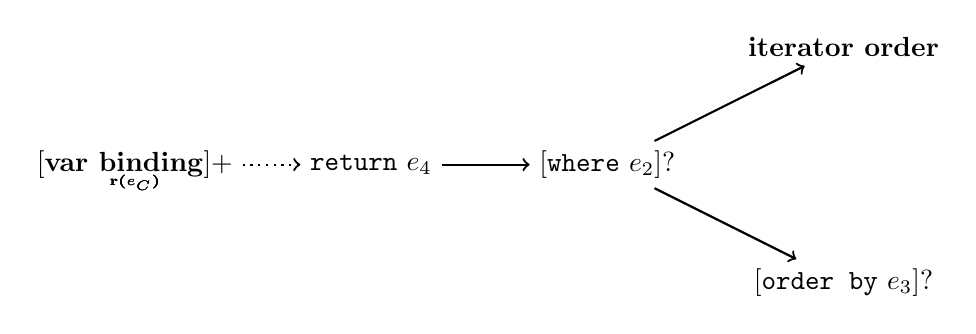
\begin{tikzpicture}

\node (bind) at (0,0) {$[$\textbf{var binding}$]+$};
\node (return) at (3,0) {\texttt{return} $e_{4}$};
\node (where) at (6,0) {$[$\texttt{where} $e_{2}]?$};
\node (itord) at (9,1.5) {\textbf{iterator order}};
\node (ordby) at (9,-1.5) {$[$\texttt{order by} $e_{3}]?$};
\draw [->,dotted,thick] (bind) to (return);
\draw [->,thick] (return) to (where) node[below,midway] {\tiny\textbf{r(}$e_{C}$\textbf{)}};
\draw [->,thick] (where) to (itord) node[below,midway] {\tiny\textbf{r(}$e_{C}$\textbf{)}};
\draw [->,thick] (where) to (ordby) node[below,midway] {\tiny\textbf{r(}$e_{C}$\textbf{)}};
\end{tikzpicture}
\label{fig:trans:TD:flworExecute}
\caption[FLWOR translation order]{Illustration of step-by-step translation of FLWOR.}
\end{figure}



Any possible iteration, ordering og filtering will be handled by other clauses than the \texttt{return} clause.
The \texttt{return} clause will just ship the evaluated version of the \texttt{return} expression forward:
\begin{equation}
\frac{}{\mbox{\texttt{return }}e_{4}}\longmapsto
\mbox{\textbf{r(}}e_{4}\mbox{\textbf{)}}
\label{rule:trans:TD:returnTaint}
\end{equation}


\subsubsection{Iterator Ordering}
The \texttt{return} clause is evaluated once for iteration for each of the iterators of the FLWOR expression. The
results of these evaluations are concatenated to form the result of the FLWOR expression. If the \texttt{return}
expression is not dependent on a iterator, its relational form will not have a representation for each
of the iterators iterations and will have to be tainted.

Because each FLWOR iterator creates a new sequence, renumbering is needed. No expression in a sibling or parent
scope of the iterator $I_{\chi}$ may be dependent on $I_{\chi}$. Thus, $\chi$ is not part of the dependencies
$I_{\chi}.\vartheta$ returned from the iterator, and the corresponding $\chi{numb}$ attribute must be removed. 

For each allready bound iterator variable $\chi$, from right to left, bound in an \texttt{for} clause,
the following translation is applied:
\begin{equation}
\frac{}{\mbox{\textbf{iterator order}}}
\longmapsto
\begin{array}{l}
\mbox{\textsf{numberate(index, [}}\beta\mbox{\textsf{, index], [}}\vartheta\mbox{\textsf{];}} \\ \quad
\mbox{\textbf{t(r(}}e_{C}\mbox{\textbf{), }}\beta\mbox{\textbf{)}}
\end{array}
\label{rule:trans:TD:itOrd}
\end{equation}

Where $\vartheta = e_{C}.\vartheta - \chi$.

From equation \ref{eq:trans:TD:taint} it is clear that a expression allready dependent on any iterator in
$\beta$ will not be re-tainted by these iterators.

The \textsf{numberate} operator will have to partition on the remaining dependencies in $\vartheta$ to seperate
the sequences returned from the iterator for all iterators the result is dependent on, as described in section
\ref{sect:trans:TD:implic}.

\begin{myExample}
Consider the query of figure \ref{fig:trans:TD:dblFor}. Notice the expression in the \texttt{return} clause ($e_1$)
is the same as $e_1$ in example \ref{ex:trans:TD:simpleSeq}.

\begin{figure}[h]
\begin{equation*}
\begin{array}{l}
\mbox{\texttt{for \$a in (10,20),}} \\
\mbox{\texttt{\phantom{abcd}\$b in (50,75)}} \\ 
\mbox{\texttt{return }}\underbrace{\mbox{\texttt{(\$a, "no")}} }_{e_{1}}
\end{array}
\end{equation*}
\caption{Example query with two iterators.}
\label{fig:trans:TD:dblFor}
\end{figure}

Expression $e_{1}$ is not depentant on $I_{\mbox{\texttt{b}}}$, and by rule \ref{rule:trans:TD:itOrd} will be
tainted by this iterator. The result of the tainting is shown in figure \ref{fig:trans:TD:final:taint}. The
expression will however not be tainted by $I_{\mbox{\texttt{a}}}$, as it is allready dependent on this iterator
(ref. equation \ref{eq:trans:TD:taint}).

\begin{figure}[h]
\centering
\subfigure[\textbf{t(r(}$e_{1}$\textbf{), \{}\texttt{b}\textbf{\})}]{
\begin{tabular}{|c|c|c|c|} \hline
$bnumb$ & $anumb$ & $index$ & $value$ \\ \hline
1 & 1 & 1 & 10 \\ \hline
1 & 2 & 1 & 20 \\ \hline
1 & 1 & 2 & \texttt{"no"} \\ \hline
1 & 2 & 2 & \texttt{"no"} \\ \hline
2 & 1 & 1 & 10 \\ \hline
2 & 2 & 1 & 20 \\ \hline
2 & 1 & 2 & \texttt{"no"} \\ \hline
2 & 2 & 2 & \texttt{"no"} \\ \hline
\end{tabular}
\label{fig:trans:TD:final:taint}
}
\qquad
\subfigure[\textbf{r(}$I_{\mbox{\texttt{a}}}$\textbf{)}]{
\begin{tabular}{|c|c|} \hline
$index$ & $value$ \\ \hline
1 & 10 \\ \hline
2 & \texttt{"no"} \\ \hline
3 & 10 \\ \hline
4 & \texttt{"no"} \\ \hline
5 & 20 \\ \hline
6 & \texttt{"no"} \\ \hline
7 & 20 \\ \hline
8 & \texttt{"no"} \\ \hline
\end{tabular}
\label{fig:trans:TD:final:rIa}
}
\caption[Example: resolving simple FLWOR]{Evaluating the query in figure \ref{fig:trans:TD:dblFor} yields the
intermediate result (a) and the final result (b).\label{fig:trans:TD:finalizeExp}}
\end{figure}

With the expression tainted with all possible iterator dependencies of the FLWOR, renumbering is the last
operation required to resolve the query. The \textsf{numberate} operator will sort the tuples first on $anumb$,
then on $bnumb$ and finally $index$ before numbering. As the FLWOR itself does not have any dependencies the
numeration will not be grouped on any attributes. The result of the query is shown in figure
\ref{fig:trans:TD:final:rIa}.
\end{myExample}

\subsubsection{Where Clause}
The W3C describes the FLWOR expression as generating a tuple stream which contains one tuple for each combination
of values bound in the expression\cite{w3c00}. In this view, the optional \texttt{where} clause serves a filter for
these tuples. The expression in the \texttt{where} clause is evaluated once for tuple. If the boolean value of this
expression is $true$, the tuple is retained, if the boolean value is $false$ the tuple is discarded.

The \texttt{where} clause can be evaluated by only selecting the iteration combinations where the \texttt{where}
expression is true. The result of this will be joined with the result of the \texttt{return} clause. If the result
from the \texttt{return} clause and the \texttt{where} expression has no common iterator dependencies, the
equi-join will have to be replaced by a cartesian product, as discussed in \ref{sect:trans:TD:implic}.

\begin{equation}
\frac{}{\mbox{\texttt{where }}e_2}\longmapsto
\begin{array}{l}
\mbox{\textsf{hhjoin([l.}}(e_{C}.\vartheta \cap e_2.\vartheta)\mbox{\textsf{], [r.}}(e_{2}.\vartheta \cap
e_{C}.\vartheta)\mbox{\textsf{], [l.value, }} \vartheta\mbox{\textsf{];}} \\ \quad
\mbox{\textbf{r(}}e_{C}\mbox{\textbf{)\textsf{;}}} \\ \quad
\mbox{\textsf{select(xqBoolean(value);}} \\ \quad \quad
\mbox{\textbf{r(}}e_{2}\mbox{\textbf{)}\textsf{))}}
\end{array}
\label{rule:trans:TD:where}
\end{equation}

Where $\vartheta = e_{C} \cup e_{2}$, and \textbf{r(}$e_{C}$\textbf{)} is the result of the translation done in
the \texttt{return} clause.

\textsf{l.}$(e_{C}.\vartheta \cap e_2.\vartheta)$ is short for
\textsf{l.}$\chi_1$\textsf{numb,\ldots,l.}$\chi_n$\textsf{numb}, where $e_{C}.\vartheta \cap e_2.\vartheta =
\left\{\chi_1,\ldots,\chi_n\right\}$.

By employing the \textsf{select} operator before the joining of the two relations the number of tuples needed to
be read to execute the join will be minimized. Further, as the \textsf{hhjoin} operator allows for declaring which
attributes to be projected, there is no need for a seperate \textsf{project} operator.

\begin{myExample}
Consider the XQuery query of figure \ref{fig:trans:TD:whereQuery}. The evaluation of $e_{1}$ is very similar to
the evaluation of $e_{1}$ of example \ref{ex:trans:TD:simpleSeq}, and the is shown in figure
\ref{fig:trans:TD:where:re1}. The \texttt{where} clause contains a comparison expression, which will be discussed
later. Figure \ref{fig:trans:TD:where:whereE} shows the result relation of the \texttt{where} expression.

\begin{figure}[h]
\centering
\begin{equation*}
\begin{array}{l}
\mbox{\texttt{for \$a in (10,20)}} \\
\mbox{\texttt{where \$a > 15}} \\
\mbox{\texttt{return}} \underbrace{\mbox{\texttt{(\$a, 14)}}}_{e_{1}}
\end{array}
\end{equation*}
\caption{A FLWOR expression with a \texttt{where} clause \label{fig:trans:TD:whereQuery}}
\end{figure}

\begin{figure}[h]
\centering
\subfigure[\textbf{r(}$e_{1}$\textbf{)}]{
\begin{tabular}{|c|c|c|} \hline
$anb$ & $idx$ & $val$ \\ \hline
1 & 1 & 10 \\ \hline
1 & 2 & 14  \\ \hline
2 & 1 & 20 \\ \hline
2 & 2 & 14  \\ \hline
\end{tabular}
\label{fig:trans:TD:where:re1}
}
\qquad
\subfigure[\textbf{r(}\texttt{\$a > 15}\textbf{)}]{
\begin{tabular}{|c|c|c|} \hline
$anb$ & $idx$ & $val$ \\ \hline
1 & 1 & $false$ \\ \hline
2 & 1 & $true$ \\ \hline
\end{tabular}
\label{fig:trans:TD:where:whereE}
}
\qquad
\subfigure[]{
\begin{tabular}{|c|c|c|} \hline
$anb$ & $idx$ & $val$ \\ \hline
2 & 1 & 20 \\ \hline
2 & 2 & 14  \\ \hline
\end{tabular}
\label{fig:trans:TD:where:intr}
}

\caption[Example: Evaluation of where clause]{Applying rule \ref{rule:trans:TD:where} on (a) and (b)
yields (c). Attribute names are shortened. \label{fig:trans:TD:whereClause}}
\end{figure}

During the evaluation of the FLWOR, the tuples in the \texttt{where} expression relation where $value$ ($val$ in
figure) is not $true$ will be removed. The result is a relation with a single tuple where $anumb$ holds the value
$2$. This result is then joined with the $e_1$ relation on $anumb$, as shown in figure
\ref{fig:trans:TD:where:intr}. Rule \ref{rule:trans:TD:itOrd} will have to be applied to complete the
evaluation of the query.
\end{myExample}


\subsubsection{Order By Clause Ordering}

As can be seen in figure \ref{fig:trans:TD:ordEBNF}, an \texttt{Order by} clause may contain several specifications on
how to order and what to order by.
\begin{figure}[h]
\begin{Verbatim}
[38] OrderByClause ::= (("order" "by") | ("stable" "order" "by")) 
                           OrderSpecList
[39] OrderSpecList ::= OrderSpec ("," OrderSpec)*
[40] OrderSpec     ::= ExprSingle OrderModifier
[41] OrderModifier ::= ("ascending" | "descending")? 
                           ("empty" ("greatest" | "least"))? 
                           ("collation" URILiteral)?
\end{Verbatim}
\label{fig:trans:TD:ordEBNF}
\caption[W3C EBNF order by clause specification]{W3C EBNF order by clause specification.}
\end{figure}

At this time, Taiting Dependencies only support a simple form of the clause. Only one \texttt{OrderSpec} is
allowed, where the expression to be sorted on will be referred to as $e_4$ -- conformant to figure
\ref{fig:trans:TD:flworExecute}. No \texttt{OrderModifier}s are allowed, and neither is the \texttt{stable}
option. This will be discussed further in sectin \ref{sect:disc:orderby}.

As with the \texttt{where} clause W3C specify the \texttt{order by} clause as operating on a tuple stream created
by the variable bindings in the FLWOR. The clause causes the stream to be reordered into a new, value-based order.
This means that the iterator dependency attributes ($\chi{numb}$) will no longer decide the composition of the
sequence returned from the FLWOR.

Firstly, to ensure that the result will have a representation for all the iterations (still valid after possible
filtering by \texttt{where} clause) of all the expressions iterators, $e_C$ is tainted with $\beta$. The
\texttt{order by} expression is evaluated and joined with the result of the tainting on their common iterator
dependencies. Lastly, this relation is renumbered according to the order of the values stemming from the
\texttt{order by} expression:

\begin{equation}
\frac{}{\mbox{\texttt{order by }}e_3}\longmapsto
\begin{array}{l}
\mbox{\textsf{project(value = l.value, }}\vartheta\mbox{\textsf{;}}\\ \quad
\mbox{\textsf{numberate(index, [r.value, index], [}}\vartheta\mbox{\textsf{];}} \\ \quad \quad
\mbox{\textsf{hhjoin([l.}}(e_{C}.\vartheta \cap e_2.\vartheta)\mbox{\textsf{], [r.}}(e_{2}.\vartheta \cap
e_{C}.\vartheta)\mbox{\textsf{],}} 
\\ \quad \quad \quad \quad \quad\mbox{\textsf{[l.value, r.value, }} \vartheta\mbox{\textsf{];}} \\ \quad \quad
\quad \mbox{\textbf{t(r(}}e_C\mbox{\textbf{), }}\beta\mbox{\textbf{)}\textsf{;}} \\ \quad \quad \quad
\mbox{\textbf{r(}}e_3\mbox{\textbf{)}\textsf{)))}}
\end{array}
\end{equation}

Where $\vartheta = (e_C.\vartheta \cup e_3.\vartheta)-\beta$, and \textbf{r(}$e_{C}$\textbf{)} is the result of
the translation done in the \texttt{where} clause if present, else the \texttt{return} clause.

As desired, all iterator dependency attributes ($\chi{numb}, \chi \in \beta$) will be projected away by the
\textsf{hhjoin} operator. An additional \textsf{project} operator is used to ensure that the $value$ returned from
the expression is the $value$ attribute of the \texttt{return} expression.

\begin{myExample}
Figure \ref{fig:trans:TD:ordQu} shows a query consisting of a FLWOR expression containing a \texttt{order by} clause.
\begin{figure}[h]
\centering
\begin{tabular}{l}
\texttt{for \$a in (4, 6, 8)} \\
\texttt{order by \$a mod 3}\\
\texttt{return \$a}\\
\end{tabular}
\label{fig:trans:TD:ordQu}
\caption{Example query with order by clause}
\end{figure}

The evaluated \texttt{order by} expression is shown in figure \ref{fig:trans:TD:ord:oExp}. How modulus expressions
are translated will be discussed later. After their evaluation, the relational representation of \texttt{order by}
expression relation and the \texttt{return} clause is joined on their common iterator dependencies,
$I_{\mbox{\texttt{a}}}$. The result of the join is shown in figure \ref{fig:trans:TD:ord:join}. Lastly, this
relation is renumbered sorted on the $r.value$ ($r.val$ in figure) attribute stemming from the \texttt{order by}
expression, as shown in figure \ref{fig:trans:TD:ord:numb}. An additional projection to rename $l.value$ to $value$
is needed to finalise the query.

\begin{figure}[h]
\subfigure[\textbf{r(}\texttt{\$a mod 3}\textbf{)}]{
\begin{tabular}{|c|c|c|} \hline
$idx$ & $anb$ & $val$ \\ \hline
1 & 1 & 1 \\ \hline
1 & 2 & 0 \\ \hline
1 & 3 & 2 \\ \hline
\end{tabular}
\label{fig:trans:TD:ord:oExp}
}
\qquad
\subfigure[]{
\begin{tabular}{|c|c|c|c|} \hline
$l.idx$ & $anb$ & $l.val$ & $r.val$ \\ \hline
1 & 1 & 4 & 1 \\ \hline
1 & 2 & 6 & 0 \\ \hline
1 & 3 & 8 & 2 \\ \hline
\end{tabular}
\label{fig:trans:TD:ord:join}
}
\qquad
\subfigure[]{
\begin{tabular}{|c|c|} \hline
$l.idx$ & $l.val$ \\ \hline
1 & 6 \\ \hline
2 & 4 \\ \hline
3 & 8 \\ \hline
\end{tabular}
\label{fig:trans:TD:ord:numb}
}


\caption{Intermediate results evaluating the query of figure
\ref{fig:trans:TD:ordQu}. (a) shows the evaluated \texttt{order by} expression. (b) shows the \texttt{order by}
expression joined with the \texttt{return} expression. (c) shows the relation in (b) renumbered. Attribute names
are shortened.\label{fig:trans:TD:orderRes}}
\end{figure}


\end{myExample}

\subsection{Arithmetic Expressions}
\label{sect:trans:TD:atrith}
W3C defines the arithmetic expressions as shown in figure \ref{fig:trans:TD:arithEBNF}\cite{w3c00}. Notice how the
specified grammar handles operator precedence. \texttt{UnaryExpr} is a decendant production of \texttt{UnionExpr}.

\begin{figure}[h]
\begin{Verbatim}
[50] AdditiveExpr       ::= MultiplicativeExpr ( ("+" | "-") 
                                MultiplicativeExpr )*
[51] MultiplicativeExpr ::= UnionExpr 
                                ( ("*" | "div" | "idiv" | "mod")
                                UnionExpr )*
[58] UnaryExpr          ::= ("-" | "+")* ValueExpr
\end{Verbatim}
\caption{The arithmetic expressions of XQuery}
\label{fig:trans:TD:arithEBNF}
\end{figure}

The translation of such expressions will have to be separated in binary and unary operators. For the binary
operators the two values to be operated on will have to be in the same relation. To ensure the values to be
operated on are from the same unique iteration (if there is any iterations at all), the relations corresponding to
the two expressions will have to be joined on their common iterator dependencies, as described in section
\ref{sect:trans:TD:implic}. Both the unary and the binary XQuery arithmetic operators accept only singleton
sequences.

\begin{equation}
\frac{}{e_1 \mbox{\texttt{ OP }} e_2}\longmapsto
\begin{array}{l}
\mbox{\textsf{project(index=1,value=FUNC(l.value,r.value),}}\vartheta\mbox{\textsf{;}} \\ \quad
\mbox{\textsf{hhjoin([l.}}(e_1.\vartheta\cap e_2.\vartheta)\mbox{\textsf{], [r.}}(e_2.\vartheta\cap e_1.\vartheta)
\mbox{\textsf{],}} 
\\ \quad \quad \quad \quad\mbox{\textsf{[r.value, l.value, }}\vartheta\mbox{\textsf{];}} \\ \quad \quad
\mbox{\textbf{r(}}e_1\mbox{\textbf{)}} \\ \quad \quad
\mbox{\textbf{r(}}e_2\mbox{\textbf{)}\textsf{))}}
\end{array}
\label{rule:trans:TD:arithmetic}
\end{equation}

Where $\vartheta = e_1.\vartheta \cup e_2.\vartheta$, \texttt{OP} will map to a MQL function replacing
\textsf{FUNC} as shown in table \ref{tab:trans:TD:binOpMap}. The projecting functionality of the
\textsf{hhjoin} operator will in this case remove the $index$ attributes and any possible $documentId$, $scope$
and $pos$ attributes.

\begin{table}[h]
\centering
\begin{tabular}{c|c}
\texttt{OP} & \textsf{FUNC} \\ \hline
\texttt{+} 	& \textsf{sum} \\
\texttt{-} 	& \textsf{subtract} \\
\texttt{*} 	& \textsf{prod} \\
\texttt{div} 	& \textsf{div} \\
\texttt{idiv} 	& \textsf{idiv} \\
\texttt{mod} 	& \textsf{mod} \\
\end{tabular}
\label{tab:trans:TD:binOpMap}
\caption{Mapping XQuery arithmetic operators to MQL functions.}
\end{table}

Considering the unary operators, the \texttt{+} operator will never have any effect, and can therefore be dropped.
The unary \texttt{-} operator will change the sign of the value it is assigned to. This is equal to multiplying
the value with $-1$:
\begin{equation}
\frac{}{\mbox{\texttt{-}}e_1}\longmapsto 
\begin{array}{l}
\mbox{\textsf{project(value = prod(-1, value);}} \\ \quad
\mbox{\textbf{r(}}e_1\mbox{\textbf{)}\textsf{)}}
\end{array}
\label{rule:trans:TD:unaryMin}
\end{equation}

\begin{myExample}
Consider the XQuery query of figure \ref{fig:trans:TD:arithQuery}. Here $e_1$ is an arithmetic expression.

\begin{figure}[h]
\centering
\begin{equation*}
\begin{array}{l}
\mbox{\texttt{for \$a in (1,2) return}} \\ \quad
\mbox{\texttt{for \$b in (3,4) return}} \\ \quad \quad
\underbrace{\mbox{\texttt{\$a + \$b}}}_{e_1}
\end{array}
\end{equation*}
\caption{Example query containting a arithmetic expression.}
\label{fig:trans:TD:arithQuery}
\end{figure}

Both \texttt{\$a} and \texttt{\$b} is translated to simple two-tuple relations by rules
\ref{rule:trans:TD:forbind} and \ref{rule:trans:TD:varRef}. As the two expressions do not have any iterator
dependencies the \texttt{hhjoin} operator of rule \ref{rule:trans:TD:arithmetic} will be treated as a cartesian
product (ref. \ref{sect:trans:TD:implic}). The cross product of the two relations are shown in figure
\ref{fig:trans:TD:aritJoin}. Lastly, the \texttt{project} operator is employed to calculate the sum for each
iteration, the result of which is shown in figure \ref{fig:trans:TD:aritEnd}.

\begin{figure}[h]
\centering
\subfigure[]{
\begin{tabular}{|c|c|c|c|}\hline
$anb$ & $bnb$ & $l.val$ & $r.val$ \\ \hline
1 & 1 & 1 & 3 \\ \hline
2 & 1 & 2 & 3 \\ \hline
1 & 2 & 1 & 4 \\ \hline
2 & 2 & 2 & 4 \\ \hline
\end{tabular}
\label{fig:trans:TD:aritJoin}
}
\qquad
\subfigure[\textbf{r(}$e_1$\textbf{)}]{
\begin{tabular}{|c|c|c|c|}\hline
$idx$ & $anb$ & $bnb$ & $val$ \\ \hline
1 & 1 & 1 & 4 \\ \hline
1 & 2 & 1 & 5 \\ \hline
1 & 1 & 2 & 5 \\ \hline
1 & 2 & 2 & 6 \\ \hline
\end{tabular}
\label{fig:trans:TD:aritEnd}
}
\caption[Results of evaluating expression $e_1$ of figure \ref{fig:trans:TD:arithQuery}.]{Results of evaluating
expression $e_1$ of figure \ref{fig:trans:TD:arithQuery}. (a) shows the result of the cross product. (b) is the
fully evaluated $e_1$. Attribute names are shortened. \label{fig:trans:TD:arithRes}}
\end{figure}

\end{myExample}

\subsection{Logical Expressions}
\label{sect:trans:TD:logical}
An XQuery logical expression is either an \texttt{and} expression or an \texttt{or} expression. If a logical
expression does not raise an error, its value is always one of the boolean values $true$ or $false$.

A logical expression is translated in a matter very similar to the arithmetic expressions. The XQuery logical
operators does however operate on the effective boolean value (see section \ref{sect:theory:xquery:basics}) rather
than the direct value. Rule \ref{rule:trans:TD:arithmetic} is valid for logical expressions, and the mapping
between the XQuery operators and the MQL functions are shown in table JEJEJEJE. As the operators require effective
boolean values, the $value$ fields will have to be run through the \textsf{xqBoolean()} function. E.g. the
following will be a part of the parameters of the \textsf{project} operator of a translated \texttt{or} expression:
\textsf{\ldots value = or(xqBoolean(l.value),xqBoolean(r.value))\ldots}.

\begin{table}[h]
\centering
\begin{tabular}{c|c}
\texttt{OP} & \textsf{FUNC} \\ \hline
\texttt{or} & \textsf{or} \\
\texttt{and} & \textsf{and} \\
\end{tabular}
\label{tab:trans:TD:logMap}
\caption{Mapping XQuery boolean operators to MQL functions}
\end{table}

For logical expressions, $e_1$\texttt{ logOp }$e_2$, $e_1$ and $e_2$ and their possible subexpressions will have
to be translated in the logical context $\Lambda$.

\subsection{Comparative Expressions}
\label{sect:trans:TD:compArit}
Comparison expressions allow two values to be compared. XQuery provides three kinds of comparison expressions,
called value comparisons, general comparisons, and node comparisons. The comparison operators as specified by W3C
are shown in figure \ref{fig:trans:TD:compEBNF}. The Tainting Dependency method does at this time not support node
comparison, as will be discussed in section \ref{sect:disc:notSupported}.

\begin{figure}[h]
\begin{Verbatim}
[61] ValueComp   ::= "eq" | "ne" | "lt" | "le" | "gt" | "ge"
[60] GeneralComp ::= "=" | "!=" | "<" | "<=" | ">" | ">="
[62] NodeComp    ::= "is" | "<<" | ">>"
\end{Verbatim}
\caption{The comparison operators of XQuery}
\label{fig:trans:TD:compEBNF}
\end{figure}

Value comparisons are used for comparing two single values. With the same premises and restrictions the rule for
translating arithmetic expressions (rule \ref{rule:trans:TD:arithmetic}) can be used to translate such comparison
expressions. The mapping between the XQuery value comparators and MQL functions can be seen in table
\ref{tab:trans:TD:valueComp}.

\begin{table}[h]
\centering
\begin{tabular}{c|c}
\texttt{OP} & \textsf{FUNC} \\ \hline
\texttt{eq} & \textsf{eq} \\
\texttt{ne} & \textsf{neq} \\
\texttt{lt} & \textsf{lt} \\
\texttt{le} & \textsf{leq} \\
\texttt{gt} & \textsf{gt} \\
\texttt{ge} & \textsf{geq} \\
\end{tabular}
\label{tab:trans:TD:valueComp}
\caption{Mapping XQuery value comparators to MQL functions}
\end{table}

General comparisons are existentially quantified comparisons that may be applied to sequences of any length. If
employing a general comparator on any pair of items consisting of one from each of the sequences yields $true$,
the comparison expression yields true. As an example, all the comparison expressions of figure
\ref{fig:trans:TD:genCompEx} evaluates to $true$.

\begin{figure}[h]
\centering
\begin{tabular}{l}
\texttt{(1, 2) = (2, 3)} \\
\texttt{(1, 2) != (2, 3)} \\
\texttt{(1, 200) < (10, 20)} \\
\texttt{(1, 200) > (10, 20)} \\
\end{tabular}
\label{fig:trans:TD:genCompEx}
\caption[Example general comparisons]{Example general comparisons: all expressions evaluate to $true$}
\end{figure}

The big difference between general and value comparisons is that the first must accomodate for sequences. This is
solved by grouping expressions' iterator dependencies, meaning that each group will contain the sequence of one
unique iteration. By defining $true$ as having a larger value than $false$, the \textsf{max()} aggregator will
identify the groups with \emph{at least} one $true$ value.

As with the arithmetic expressions, the relational representation of the two operands is joined on their common
dependencies to ensure that both values are from the same iteration.

\begin{equation}
\frac{}{e_1\mbox{\texttt{ OP }}e_2}\longmapsto
\begin{array}{l}
\mbox{\textsf{project(index = 1, value=max, }}\vartheta \textsf{;} \\ \quad
\mbox{\textsf{group((}}\vartheta\mbox{\textsf{), max(value);}} \\ \quad \quad
\mbox{\textsf{project(value=FUNC(r.value,l.value),}}\vartheta\mbox{\textsf{;}} \\ \quad \quad \quad
\mbox{\textsf{hhjoin([l.}}(e_1.\vartheta\cap e_2.\vartheta)\mbox{\textsf{], [r.}}(e_2.\vartheta\cap e_1.\vartheta)
\mbox{\textsf{],}} 
\\ \quad \quad \quad \quad \quad \quad\mbox{\textsf{[l.value, r.value, }}\vartheta\mbox{\textsf{];}} \\ \quad \quad
\quad \quad \quad \mbox{\textbf{r(}}e_1\mbox{\textbf{)}} \\ \quad \quad \quad \quad \quad
\mbox{\textbf{r(}}e_2\mbox{\textbf{)}\textsf{))))}}
\end{array}
\label{rule:trans:TD:comparative}
\end{equation}

Where $\vartheta = e_1.\vartheta \cup e_2.\vartheta$. \texttt{OP} wil map to a MQL function replacing
\textsf{FUNC} as shown in table \ref{tab:trans:TD:genCompMap}. 

The result of a general comparison is always a singleton sequence, thus it is safe to project in an $index$
attribute with the value $1$. The $index$ and possible $documentId$, $scope$ and $pos$ attributes are left out of
the project list of the \textsf{hhjoin} operator.

\begin{table}[h]
\centering
\begin{tabular}{c|c}
\texttt{OP} & \textsf{FUNC} \\ \hline
\texttt{=} & \textsf{eq} \\
\texttt{!=} & \textsf{neq} \\
\texttt{<} & \textsf{lt} \\
\texttt{<=} & \textsf{leq} \\
\texttt{>} & \textsf{gt} \\
\texttt{>=} & \textsf{geq} \\
\end{tabular}
\label{tab:trans:TD:genCompMap}
\caption{Mapping XQuery general comparators to MQL functions.}
\end{table}

\begin{myExample}
Figure \ref{fig:trans:TD:genCompQu} shows a simple XQuery query with a general comparison expression, $e_1$.
\begin{figure}[h]
\centering
\begin{equation*}
\begin{array}{l}
\mbox{\texttt{for \$a in (10, 20) return}} \\ \quad
\underbrace{\mbox{\texttt{\$a > (5, 15)}}}_{e_1}
\end{array}
\end{equation*}
\caption{Example query with a general comparison expression \label{fig:trans:TD:genCompQu}}
\end{figure}
 
Because the operands of the \texttt{>} operator have no common iterator dependencies, the cartesian product of the
two relations are calculated, as seen in figure \ref{fig:trans:TD:gen:join}. After the inner \textsf{project}
operator is employed, the result will be as in figure \ref{fig:trans:TD:gen:projGr}. The double line illustrates
the grouping on $anumb$ ($anb$ in the figure). The maximum value of $value$ for each group is calculated and the
attributes are renamed, which gives the relation of figure \ref{fig:trans:TD:gen:end}.

\begin{figure}[h]
\centering
\subfigure[]{
\begin{tabular}{|c|c|c|} \hline
$anb$ & $l.val$ & $r.val$ \\ \hline
1 & 10 & 5 \\ \hline
1 & 10 & 15 \\ \hline
2 & 20 & 5 \\ \hline
2 & 20 & 15 \\ \hline
\end{tabular}
\label{fig:trans:TD:gen:join}
}
\qquad
\subfigure[]{
\begin{tabular}{|c|c|} \hline
$anb$ & $val$ \\ \hline
1 & $true$ \\ \hline
1 & $false$ \\ \hline \hline
2 & $true$ \\ \hline
2 & $true$ \\ \hline
\end{tabular}
\label{fig:trans:TD:gen:projGr}
}
\qquad
\subfigure[\textbf{r(}$e_1$\textbf{)}]{
\begin{tabular}{|c|c|c|} \hline
$idx$ & $anb$ & $val$ \\ \hline
1 & 1 & $true$ \\ \hline
1 & 2 & $true$ \\ \hline
\end{tabular}
\label{fig:trans:TD:gen:end}
}
\caption[Results of evaluating $e_1$ in figure \ref{fig:trans:TD:genCompQu}]{Results of evaluating expression $e_1$
in figure \ref{fig:trans:TD:genCompQu}. (a) The relations of the operands joined. (b) Each combination of the
sequences evaluated. Double line illustrates grouping. (c) The final result. Attribute names are shortened.
\label{fig:trans:TD:genCompRes}}
\end{figure}
 
\end{myExample}

\section{Conditional Expressions}
\label{sect:trans:TD:ifThenElse}
XQuery supports a conditional expression based on the keywords \texttt{if}, \texttt{then}, and \texttt{else}. The
expression is defined by W3C as seen in figure \ref{fig:trans:TD:condEBNF}.

\begin{figure}[h]
\begin{Verbatim}
[45] IfExpr ::= "if" "(" Expr ")" "then" ExprSingle 
                    "else" ExprSingle
\end{Verbatim}
\label{fig:trans:TD:condEBNF}
\caption{W3C EBNF conditional expression specification.}
\end{figure}

The expression following the \texttt{if} keyword is called the test expression, and the expressions following the
\texttt{then} and \texttt{else} keywords are called the \texttt{then}-expression and \texttt{else}-expression,
respectively. If the effective boolean value of the test expression evaluates to $true$, the
\texttt{then}-expression is returned, if it evaluates to $false$ the \texttt{else}-expression is returned.

Conditional expressions are translated by adding an attribute $alt$ with the value $1$ the
\texttt{then}-expression relation and the relational representation of the \texttt{else}-expression with the same
attribute but with value $2$. These two relations are then spliced together with a \textsf{union} operator. If the
relations have disjoint dependencies, they will have to be tainted first.

The result of the \textsf{union} operation is then joined with the relational representation of the test
expression on their common dependencies. Lastly, a \textsf{select} operator is employed on this relation to select
the tuples where $alt$ is $1$ if the $value$ field from the test expression evaluates to $true$, or $alt$ is $2$
if it does not.

\begin{equation}
\begin{array}{c}
\frac{}{\mbox{\texttt{if }}e_1\mbox{\texttt{ then }}e_2\mbox{\texttt{ else }}e_3} \\
\longmapsto \\
\begin{array}{l}
\mbox{\textsf{project(value = l.value, }}\vartheta\mbox{\textsf{;}} \\ \quad
\mbox{\textsf{select(ifthenelse(xqBoolean(r.value), eq(alt,1), eq(alt,2));}} \\ \quad \quad
\mbox{\textsf{hhjoin([}}((e_2.\vartheta \cup e_3.\vartheta)\cap e_1.\vartheta)\mbox{\textsf{],
[}}(e_1.\vartheta\cap (e_2.\vartheta\cup e_3.\vartheta))
\mbox{\textsf{],}} 
\\  \quad \quad \quad \quad \quad\mbox{\textsf{[l.value, r.value, }}\vartheta\mbox{\textsf{];}}\\\quad\quad\quad
\mbox{\textsf{union(}} \\ \quad\quad\quad\quad
\mbox{\textsf{project(alt=1, value, }}(e_2.\vartheta \cup e_3.\vartheta)\mbox{\textsf{,}}\\\quad\quad\quad\quad\quad
\mbox{\textbf{t(r(}}e_2\mbox{\textbf{), }}e_3.\vartheta\mbox{\textbf{)}\textsf{);}} \\ \quad\quad\quad\quad
\mbox{\textsf{project(alt=2, value, }}(e_3.\vartheta\cup e_2.\vartheta)\mbox{\textsf{,}}\\\quad\quad\quad\quad\quad
\mbox{\textbf{t(r(}}e_3\mbox{\textbf{), }}e_2.\vartheta\mbox{\textbf{)}\textsf{));}}\\\quad\quad\quad
\mbox{\textbf{r(}}e_1\mbox{\textbf{)}\textsf{)))}}
\end{array}
\end{array}
\label{rule:trans:TD:conditional}
\end{equation}

Where $\vartheta = e_1.\vartheta \cup e_2.\vartheta \cup e_3.\vartheta$. $index$ and possible $documentId$, $pos$
and $scope$ attributes will follow $value$ as described in \ref{sect:trans:TD:basics}.

\begin{myExample}
\begin{figure}[h]
\centering
\begin{equation*}
\begin{array}{l}
\mbox{\texttt{for \$a in (10, 20) return}} \\ \quad
\mbox{\texttt{for \$b in (5, 15) return}} \\ 
e_1 \left\{\begin{array}{l}
           \mbox{\texttt{if(\$b > \$a) then}} \\ \quad
           \mbox{\texttt{\$a}} \\ 
           \mbox{\texttt{else}} \\ \quad
           \mbox{\texttt{\$b}}
           \end{array}\right.
\end{array}
\end{equation*}
\caption{Example query containing a conditional expression \label{fig:trans:TD:condQue}}
\end{figure}

The query of figure \ref{fig:trans:TD:condQue} contains a conditional expression $e_1$. First the
\texttt{then}-expression and the \texttt{else}-expression are tainted with eachothers iterator dependencies. The
result of the tainting is shown in figure \ref{fig:trans:TD:inter1:taint}. Then the two relations are augmented
with the $alt$ attribute and spliced together with an \textsf{union} operator to make the relation depicted in
figure \ref{fig:trans:TD:inter1:union}.

\begin{figure}[h]
\centering
\subfigure[]{
\begin{tabular}{|c|c|c|c|} \hline
$bnb$ & $anb$ & $val$ \\ \hline
1 & 1 & 10 \\ \hline
1 & 2 & 20 \\ \hline
2 & 1 & 10 \\ \hline
2 & 2 & 20 \\ \hline
\end{tabular}
\label{fig:trans:TD:inter1:taint}
}
\phantom{A}
\subfigure[]{
\begin{tabular}{|c|c|c|c|} \hline
$alt$ & $bnb$ & $anb$ & $val$ \\ \hline
1 & 1 & 1 & 10 \\ \hline
1 & 1 & 2 & 20 \\ \hline
1 & 2 & 1 & 10 \\ \hline
1 & 2 & 2 & 20 \\ \hline
2 & 1 & 1 & 5 \\ \hline
2 & 2 & 1 & 15 \\ \hline
2 & 1 & 2 & 5 \\ \hline
2 & 2 & 2 & 15 \\ \hline
\end{tabular}
\label{fig:trans:TD:inter1:union}
}
\phantom{A}
\subfigure[]{
\begin{tabular}{|c|c|c|} \hline
$anb$ & $bnb$ & $val$ \\ \hline
1 & 1 & $false$ \\ \hline
2 & 1 & $false$ \\ \hline
1 & 2 & $true$ \\ \hline
2 & 2 & $false$ \\ \hline
\end{tabular}
\label{fig:trans:TD:inter1:test}
}
\caption[Intermediate results of evaluating $e_1$ in figure \ref{fig:trans:TD:condQue}.]{Intermediate results of
evaluating $e_1$ in figure \ref{fig:trans:TD:condQue}. (a) The \texttt{then}-expresion tainted with $I_{\mbox{\texttt{b}}}$ (b) The \texttt{then}-expression and the
\texttt{else}-expression augmented with an $alt$ attribute and spliced together. (c) The test expression.
Attribute names are shortened. $index$ attribute is left out. \label{fig:trans:TD:inter1}}
\end{figure}

The result of the \textsf{union} operation is then joined with the test expression (figure
\ref{fig:trans:TD:inter1:test}) on their common dependencies ($anumb$ and $bnumb$) to form the relation in figure
\ref{fig:trans:TD:condRes:join}. From this relation, only the tuples where $alt$ has the value 1 and $r.val$ is
$true$ or $alt$ has the value 2 and $r.val$ is $false$ are selected. The result of the selection after the final
renaming is shown in figure \ref{fig:trans:TD:condRes:res}.

\begin{figure}[h]
\centering
\subfigure[]{
\begin{tabular}{|c|c|c|c|c|} \hline
$alt$ & $bnb$ & $anb$ & $l.val$ & $r.val$ \\ \hline
1 & 1 & 1 & 10 & $false$ \\ \hline
2 & 1 & 1 & 5 & $false$ \\ \hline
1 & 2 & 1 & 10 & $true$ \\ \hline
2 & 2 & 1 & 15 & $true$ \\ \hline
1 & 1 & 2 & 20 & $false$ \\ \hline
2 & 1 & 2 & 5 & $false$ \\ \hline
1 & 2 & 2 & 20 & $false$ \\ \hline
2 & 2 & 2 & 15 & $false$ \\ \hline
\end{tabular}
\label{fig:trans:TD:condRes:join}
}
\qquad
\subfigure[]{
\begin{tabular}{|c|c|c|} \hline
$bnb$ & $anb$ & $val$ \\ \hline
1 & 1 & 5 \\ \hline
2 & 1 & 10 \\ \hline
1 & 2 & 5 \\ \hline
2 & 2 & 15 \\ \hline
\end{tabular}
\label{fig:trans:TD:condRes:res}
}
\caption[Evaluating $e_1$ in figure \ref{fig:trans:TD:condQue}.]{Evaluating $e_1$ in figure
\ref{fig:trans:TD:condQue}. (a) The test expression joined with the union of the \texttt{then}- and
\texttt{else}-expression. (b) $e_1$ fully evaluated. Attribute names are shortened. $index$ attribute is omitted.
\label{fig:trans:TD:condRes} }
\end{figure}

\end{myExample}



\section{Path expressions and predicates}
\label{sect:trans:TD:pathNpred}

XQuery implement XPath 2.0 path expressions and predicates as described in section
\ref{sect:theory:xquery:PathExpressions} and \ref{sect:theory:xquery:Predicates}. In this section we will present
a method for translating some of these expressions into MQL relational algebra.

For the translations in this section to be correct we assume the tuples returned from a scope lookup in the
hypothetical \textsf{valocc}-index (see Section \ref{sect:method:mql} on page \pageref{sect:method:mql}) will have
information of the scope it self in the $scope$ attribute, and the contents of the scope in an $value$ attribute.
E.g.\ a lookup of \textsf{\$c} (the \textsf{\$}-sign indicates it is a scope) in this index may return a tuple
with \textsf{a[1].b[2].c[1]} as its $scope$ value.

The tuples returned from a lookup in the value occurence index will have to be ordered according to document
order. This order will have to hold even after the result is run through a \textsf{scope}

The concept of the context item is important in this section, and is by the W3C defined as follows\cite{w3c00}:
\begin{quote}
[Definition: The \textbf{context item} is the item currently being processed. An item is either an atomic value or
a node.][\ldots] The context item is returned by an expression consisting of a single dot (\texttt{.}). When an
expression $e_1$\texttt{/}$e_2$ or $e_1$\texttt{[}$e_2$\texttt{]} is evaluated, each item in the sequence obtained
by evaluating $e_1$ becomes the context item in the inner focus for an evaluation of $e_2$.
\end{quote}

\subsection{Path expressions}
\label{sect:trans:TD:pathExprs}
A path expression consists of a series of one or more steps, separated by ``/'' or ``//'', and optionally beginning
with ``/'' or ``//''.  Each step is either a axis step or a filter expression, and a axis step consist of a axis
and a node test. This can be seen from the excerpt of the W3C XQuery
specification in Figure \ref{fig:trans:TD:pathEBNF}. A node test can be either a kind test or a name test, we will focus on the latter. 

\begin{figure}[h]
\begin{Verbatim}
[68] PathExpr        ::= ("/" RelativePathExpr?)
                       | ("//" RelativePathExpr)
                       | RelativePathExpr
[69] RelativePathExpr::= StepExpr (("/" | "//") StepExpr)*
[70] StepExpr        ::= FilterExpr | AxisStep
[71] AxisStep        ::= (ReverseStep | ForwardStep) PredicateList
[72] ForwardStep     ::= (ForwardAxis NodeTest) | AbbrevForwardStep
[75] ReverseStep     ::= (ReverseAxis NodeTest) | AbbrevReverseStep
\end{Verbatim}
\caption{Path expressions as specified by W3C\cite{w3c00} \label{fig:trans:TD:pathEBNF}}
\end{figure}
The semantics of such expressions reading from left to right, is that the result of one step expression is used as
input for the next. Within one step expression, the result from the preceding step will first be used as input for the
axis expression. The result of this will be filtered by a name or kind test, before this again is filtered by
possible predicates.

Step expressions can be abbreviated. If the axis name is omitted from an axis step, the default axis is
\texttt{child}. \texttt{decendant-or-self} can be replaced by using ``\texttt{//}'' istead of ``\texttt{/}''
between the steps. \texttt{@} is an abbreviation of \texttt{attribute::}. We will only present translation of
unabbreviated syntax.

To accomodate for the context item, the result of each step of a path expression will be stored on the symbol
table as \textbf{dot} -- each time replacing the the last entry. The context item, and references to it will be
treated as iterator dependencies. The attribute corresponding to a dependency on \textbf{dot} is $dotNumb$. No
expression not within the path expression can be dependent on \textbf{dot},
which is why \textbf{dot} will not be part of the dependencies $\vartheta$ returned. A general path expression is translated in the following manner:

\begin{equation}
\frac{}{[\mbox{\texttt{/}}]e_1\mbox{\texttt{/}}\ldots\mbox{\texttt{/}}e_n} \longmapsto
\begin{array}{l}
\mbox{\textbf{put(dot, t(r(}}e_1\mbox{\textbf{), \{dot\}))}} \\
\qquad \qquad \vdots \\
\mbox{\textbf{put(dot, t(r(}}e_n\mbox{\textbf{), \{dot\}))}} \\
\mbox{\textsf{numberate(index, [dotNumb, index], [}}\vartheta\mbox{\textsf{];}} \\ \quad
\mbox{\textbf{get(dot)}\textsf{)}}
\end{array}
\label{rule:trans:TD:pathExpr}
\end{equation} 

Where $\vartheta = (e_n.\vartheta-$\textbf{dot}$)$. Axis step expressions are all dependent on the context item and
will take no effect of the tainting. Tainting is used in this context to ensure filter expressions to be evaluated
correctly. The $\vartheta$ piggybacking the tree in the symbol table will contain \textbf{dot}, as with
the iterator variables.

A general step expression, axis + name test, can be translated like this:
\begin{equation}
\begin{array}{c}
\frac{}{\displaystyle \texttt{AXIS::}QName_1} \\ 
\longmapsto \begin{array}{c}\mbox{\tiny } \\ \mbox{\tiny } \end{array} \\
\begin{array}{l}
\mbox{\textsf{project(docId, index, value, pos, scope, }}\vartheta\mbox{\textsf{;}} \\ \quad
\mbox{\textsf{numberate(dotNumb, [dotNumb, subIdx], [}}(\vartheta-\mbox{\textbf{dot}})\mbox{\textsf{];}} \\
\quad\quad 
\mbox{\textsf{numberate(index, [index], [}}\vartheta\mbox{\textsf{];}} \\ \quad\quad\quad
\mbox{\textsf{select(isFUNC(scope, lsc);}} \\ \quad \quad\quad\quad
\mbox{\textsf{hhjoin([docId],[docId],}}
\mbox{\textsf{[lsc=l.scope,subIdx=r.index,r.value,}}\vartheta\mbox{\textsf{];}}\\
\quad\quad\quad\quad\quad \mbox{\textbf{get(dot)}\textsf{;}} \\ \quad \quad\quad \quad\quad
\mbox{\textsf{numberate(index, [], [];}}\\ \quad\quad\quad\quad\quad\quad
\mbox{\textsf{index(valocc;}} \\ \quad\quad\quad\quad\quad\quad\quad
\mbox{\textsf{lookup(\$}}QName_1\mbox{\textsf{))))))))}}
\end{array}
\end{array}
\label{rule:trans:TD:pathStep}
\end{equation}

Where $\vartheta$ is the $\vartheta$ returned from \textbf{get(dot)}, $QName_1$ is any XML-qualified name.
\textsf{r.value} is short for \textsf{value = right.value, index = right.index, \ldots etc}, and \textsf{docId} is
short for \textsf{documentId}. \texttt{AXIS} will map to an MQL funciton \textsf{isFUNK} as described in table
\ref{tab:trans:TD:axisMap}. To ensure correct ordering, the order of the tuples returned from the \textsf{lookup}
operator must be the same as the order of the tuples received by the \textsf{numberate} operator. 

\begin{table}[h]
\centering
\begin{tabular}{c|c}
\texttt{AXIS} & \textsf{isFUNC} \\ \hline
\texttt{child} & \textsf{isChild} \\
\texttt{descendant} & \textsf{isDescendant} \\
\texttt{attribute} & \textsf{isChild}$^{*}$ \\
\texttt{self} & \textsf{isSelf} \\
\texttt{descendant-or-self} & \textsf{isDescendantOrSelf} \\
\texttt{following} & \textsf{isFollowing} \\
\texttt{following-sibling} & \textsf{isFollowingSibling} \\
\texttt{parent} & \textsf{isParent} \\
\texttt{ancestor} & \textsf{isAncestor} \\
\texttt{ancestor-or-self} & \textsf{isAncestorOrSelf} \\
\texttt{preceding} & \textsf{isPreceding} \\
\texttt{preceding-sibling} & \textsf{isPrecedingSibling} 
\end{tabular}
\caption{Mapping between XQuery axes and MQL functions. \label{tab:trans:TD:axisMap}}
\end{table}

\textit{$^{*}$For the \texttt{attribute} axis the parameter to \textsf{lookup}
will have a \textsf{\$@}-prefix instead of the \textsf{\$}-prefix described in
the rule.}

The relation after the join will contain to copies of the $index$ attribute stemming from the lookup, $index$ and
$subIdx$. This is because the \textsf{numberate} operator will remove the attributes specified in the sort list.
The next to last \textsf{numberate} operator will number the tuples according to the document order, but among
others partition on its dependency of the context item. This numbering is necessary to solve e.g.\ numeric
predicates. The last \textsf{numberate} operator will update the $dotNumb$ field as it is possible that the axis
step do not match the items from the last step in a 1:1 ratio.

\begin{myExample}
Consider the excerpt of a XML-document of Figure \ref{fig:trans:TD:pathExXml}.
The subscript numbers are used to differentiate the different elements with same names, and are not a part of the names. Further, let a non-iterator
variable \texttt{\$a} be bound to a sequence of the \texttt{A}-nodes of the figure, but \emph{not} in document
order. An illustration of the relational representation of \texttt{\$a} as it is stored as the context item in the
symbol table is shown in Figure \ref{fig:trans:TD:pathEx:varA}. The $val$ attribute indicates which XML-node is
represented and the $scope$-attribute indicates the scope of this element. Figure \ref{fig:trans:TD:pathQu} shows
an excerpt of a query referring to the variable \texttt{\$a}. \begin{figure}[h!]
\centering
\texttt{\ldots\$a/child::B/\ldots}
\caption{Example XQuery path expression \label{fig:trans:TD:pathQu}}
\end{figure} 

\begin{figure}[h]
\centering
\begin{equation*}
\begin{array}{l}
\qquad \qquad \vdots \\
\mbox{\texttt{<A}}_{1}\mbox{\texttt{>}} \\ \quad
\mbox{\texttt{<B}}_{1}\mbox{\texttt{/>}}\mbox{\texttt{<B}}_{2}\mbox{\texttt{/>}} \\
\mbox{\texttt{</A}}_{1}\mbox{\texttt{>}} \\
\mbox{\texttt{<A}}_{2}\mbox{\texttt{>}} \\ 
\mbox{\texttt{</A}}_{2}\mbox{\texttt{>}} \\
\mbox{\texttt{<A}}_{3}\mbox{\texttt{>}} \\ \quad
\mbox{\texttt{<B}}_{3}\mbox{\texttt{/>}}\mbox{\texttt{<B}}_{4}\mbox{\texttt{/>}}\mbox{\texttt{<B}}_{5}\mbox{\texttt{/>}}
\\ \mbox{\texttt{</A}}_{3}\mbox{\texttt{>}} \\
\qquad \qquad \vdots
\end{array}
\end{equation*}
\caption[Excerpt of example XML-document.]{Excerpt of example XML-document. The
subscript numbers indicate the instance of the elements, and are not part of the QName \label{fig:trans:TD:pathExXml}}
\end{figure}

First, a lookup of \texttt{\$B} (where \texttt{\$} indicates to find a scope/node, not a word) is done in the
value occurence index. The result of this is numerated by a \textsf{numberate}-operator, as illustrated in figure
\ref{fig:trans:TD:pathEx:luB}. The $index$-attribute ($idx$ in the figure) now holds the document-order of the
\texttt{B}-nodes. As there may be more \texttt{B}-nodes in the document, the $index$ attribute may not start
at the value 1 for the tuples relevant to the query.

\begin{figure}[h]
\centering
\subfigure[\textbf{r(}\texttt{\$a}\textbf{)}]{
\begin{tabular}{|c|c|c|}  \hline
$dNb$ & $val$ & $scope$ \\ \hline
1 & \texttt{A}$_{2}$ & \textsf{..{A}[2]} \\ \hline
2 & \texttt{A}$_{3}$ & \textsf{..{A}[3]} \\ \hline 
3 & \texttt{A}$_{1}$ & \textsf{..{A}[1]} \\ \hline
\end{tabular}
\label{fig:trans:TD:pathEx:varA}
}
\qquad
\subfigure[]{
\begin{tabular}{|c|c|c|}  \hline
$idx$ & $val$ & $scope$ \\ \hline
$\ldots$ & \texttt{\ldots} & \textsf{\ldots} \\ \hline
5 & \texttt{B}$_{1}$ & \textsf{..{A}[1].B[1]} \\ \hline
6 & \texttt{B}$_{2}$ & \textsf{..{A}[1].B[2]} \\ \hline
7 & \texttt{B}$_{3}$ & \textsf{..{A}[3].B[1]} \\ \hline
8 & \texttt{B}$_{4}$ & \textsf{..{A}[3].B[2]} \\ \hline
9 & \texttt{B}$_{5}$ & \textsf{..{A}[3].B[3]} \\ \hline
$\ldots$ & \texttt{\ldots} & \textsf{\ldots} \\ \hline  
\end{tabular}
\label{fig:trans:TD:pathEx:luB}
}
\caption[Evaluating the expression of Figure \ref{fig:trans:TD:pathQu}]{Illustration of results evaluating the
expression in Figure \ref{fig:trans:TD:pathQu}. (a) The variable \texttt{\$a}.
(b) Excerpt of a lookup on the term \textsf{\$B}, and the following numbering. Some attribute names are shortened. $val$ attribute indicates which
XML-element is represented in the tuple.
\label{fig:trans:TD:pathEx}}
\end{figure}

The result of the lookup will be joined with the context item relation on their $documentId$-attribute. As we
assume only one XML-document, this attribute is omitted from our example. A \textsf{select} operator is applied to
the result of the join to prune the relation. Only the tuples where the $scope$ attribute stemming from the lookup
defines a scope which is the child scope (as defined by the MQL function
\textsf{isChild()} in Section \ref{sect:method:marsAddedOperators}) of the scope defined by the $scope$-attribute stemming from the
\texttt{\$a} relation (called $lsc$). After the selection the result will be as illustrated in figure
\ref{fig:trans:TD:pathEx:joinSel}. The copy of the $index$ column is not shown.

\begin{figure}[h]
\centering
\subfigure[]{
\begin{tabular}{|c|c|c|c|c|} \hline
$dNb$ & $idx$ & $val$ & $scope$ & $lsc$ \\ \hline
2 & 9 & \texttt{B}$_{5}$ & \textsf{..{A}[3].B[3]} & \textsf{..{A}[3]} \\ \hline
2 & 8 & \texttt{B}$_{4}$ & \textsf{..{A}[3].B[2]}& \textsf{..{A}[3]} \\ \hline
2 & 7 & \texttt{B}$_{3}$ & \textsf{..{A}[3].B[1]}& \textsf{..{A}[3]} \\ \hline 
3 & 5 & \texttt{B}$_{1}$ & \textsf{..{A}[1].B[1]} & \textsf{..{A}[1]} \\ \hline
3 & 6 & \texttt{B}$_{2}$ & \textsf{..{A}[1].B[2]} & \textsf{..{A}[1]} \\ \hline
\end{tabular}
\label{fig:trans:TD:pathEx:joinSel}
}
\quad
\subfigure[]{
\begin{tabular}{|c|c|c|c|} \hline
$dNb$ & $idx$ & $val$ & $scope$ \\ \hline
1 & 1 & \texttt{B}$_{3}$ & \textsf{..{A}[3].B[1]}\\ \hline 
2 & 2 & \texttt{B}$_{4}$ & \textsf{..{A}[3].B[2]}\\ \hline
3 & 3 & \texttt{B}$_{5}$ & \textsf{..{A}[3].B[3]}\\ \hline
4 & 1 & \texttt{B}$_{1}$ & \textsf{..{A}[1].B[1]}\\ \hline
5 & 2 & \texttt{B}$_{2}$ & \textsf{..{A}[1].B[2]}\\ \hline
\end{tabular}
\label{fig:trans:TD:pathEx:done}
}
\caption[Further evaluation of the path expression]{Further evaluation of the path expression in figure
\ref{fig:trans:TD:pathQu}. (a) The result of the selection of the joining of \textbf{r(}\texttt{\$a}\textbf{)} and
the numerated result of the lookup of \textsf{\$B}. (b) Renumbering an projection on the relation of (a). Some
attribute names are shortened.}
\end{figure}

Finally, numbering is employed two times, followed by a projection removing the last attributes stemming from the
context item relation. The result of the expression is illustrated in Figure \ref{fig:trans:TD:pathEx:done}.

\end{myExample}

\subsection{Predicates}
\label{sect:trans:TD:predicates}
A predicate consists of an expression, called a predicate expression, which evaluates to a boolean value. The
expression assigned the predicate is called a predicated expression. A predicate serves to filter a sequence,
retaining the items where the expression evaluates to $true$ and discarding all other. In the case of multiple
adjacent predicates, the predicates are applied from left to right, and the result of applying each predicate
serves as the input sequence for the following predicate. If the value of the predicate expression is a singleton
atomic value of a numeric type, the predicate truth value is $true$ if the value of the predicate expression is
equal to the position of the context item within the input sequence.

When entering a predicate the relational algebra tree corresponding to the expression assigned to the predicate is
stored as \textbf{dot}, containing a copy of $dotNumb$ called $sprDotNumb$. The reason for the copy is to ensure
that the predicate is applied to the right context item of the predicated expression. If the predicate
expression contains a path expression, it may update the $dotNumb$ fields, but $sprDotNumb$ will always correspond
to the right context item outside the predicate. The predicate expression is then evaluated, and joined with
the relational representation of predicated expression on their common dependencies. If the context item is
referred to within the predicate, the relations will have to be joined on $sprDotNumb$ from the predicate
expression and $index$ from the predicated expression aswell. The context item may be referred to explicitly with
the dot-operator (.), or implicitly through a relative path expression. When evaluating path expressions it is
important to note that predicates have higher precedence than the / (step expression separator). As the predicate
may remove items, renumbering is needed:

\begin{equation}
\frac{}{e_1\mbox{\texttt{[}}e_2\mbox{\texttt{]}}}\longmapsto
\begin{array}{l}
\mbox{\textsf{project(index, value = l.value, }}\vartheta\mbox{\textsf{;}} \\ \quad
\mbox{\textsf{numberate(index, [index], [}}\vartheta\mbox{\textsf{];}} \\ \quad\quad
\mbox{\textsf{select(ifthenelse(isNumber(pred),}}
\mbox{\textsf{eq(index,pred), xqBoolean(pred));}} \\\quad\quad\quad
\mbox{\textsf{hhjoin([}}(e_1.\vartheta\cap e_2.\vartheta)\mbox{\textsf{], [}}(e_2.\vartheta\cap e_1.\vartheta)\mbox{\textsf{],}} 
\mbox{\textsf{[l.value,pred,}}\vartheta\mbox{\textsf{];}}
\\\quad\quad\quad\quad
 \mbox{\textbf{r(}}e_1\mbox{\textbf{)}\textsf{;}} \\\quad\quad\quad\quad
\mbox{\textbf{B(r(}}e_2\mbox{\textbf{)}\textsf{))))}} \\
\end{array}
\label{rule:trans:TD:predicate}
\end{equation}

Where $\vartheta=(e_1.\vartheta \cup e_2.\vartheta)-$\textbf{sprDot}. The fields of the left relation in the join
will follow \textsf{l.value} as described in Section \ref{sect:trans:TD:basics}. The final \textsf{project}
operator will restore the names of these attributes.

As described earlier, before translation of the expression the context item will be store in the symbol table:
\begin{equation*}
\begin{array}{l}
\mbox{\textbf{put(dot,}} \\ \quad
\mbox{\textsf{project(sprDotNumb=index, dotNumb=index, index=1, value, }}\vartheta\mbox{\textsf{;}} \\ \quad\quad
\mbox{\textbf{r(}}e_1\mbox{\textbf{)}\textsf{)}\textbf{)}}.
\end{array} 
\end{equation*}
However, if \textbf{dot} $\in e_1.\vartheta$, it will have to be stored in the following way:
\begin{equation*}
\begin{array}{l}
\mbox{\textbf{put(dot,}} \\ \quad
\mbox{\textsf{project(sprDotNumb=dotNumb, dotNumb, index=1, value, }}\vartheta\mbox{\textsf{;}} \\ \quad\quad
\mbox{\textbf{r(}}e_1\mbox{\textbf{)}\textsf{)}\textbf{)}}.
\end{array} 
\end{equation*}
In both cases, attributes not explicitly mentioned will follow $value$ and the $\vartheta$ piggybacking the tree
stored in the symbol table will be $($\textbf{dot} $\cup$ \textbf{sprDot} $\cup$ $e_1.\vartheta)$. The reason why
there is both a $sprDotNumb$ and $dotNumb$ in the same relation is because $dotNumb$ may be updated if the predicate is
a path expression (ref Section \ref{sect:trans:TD:pathExprs}).

If $e_2$ is dependent on \textbf{sprDot} -- meaning the predicate utilises the context item -- the relations will
be joined on \textbf{r(}$e_1$\textbf{).}$dotNumb$ \textsf{=} \textbf{r(}$e_2$\textbf{).}$sprDotNumb$ (as opposed
to \textbf{r(}$e_1$\textbf{).}$index$ \textsf{=} \textbf{r(}$e_2$\textbf{).}$sprDotNumb$ if it is not), as well as
their common dependencies.

\begin{myExample}
Consider the XQuery query of Figure \ref{fig:trans:TD:predQu}. In this query the predicate expression is dependent
on the context item.
\begin{figure}[h]
\centering
\verb!(2, 3, 4, 5)[. mod 2 = 0]!
\caption{Example query with a predicate. \label{fig:trans:TD:predQu}}
\end{figure}

The predicated sequence is illustrated in \ref{fig:trans:TD:pred:seq}. As it is not dependent on \textbf{dot} its
$index$ attribute will be renamed to $sprDotNumb$ ($sdNb$ in the figure) before it is stored in the symbol table. A
reference to the context item is like a reference to a variable, and the predicate expression evaluates to the
relation illustrated in Figure \ref{fig:trans:TD:pred:predEx}. The two relations only joined together on $index$
from the predicated expression and $sprDotNumb$ from the predicate expression, as they do not have any other
dependencies. Further, as the predicate expression does not evaluate to a numeric type, only the tuples where
$pred$ is $true$ are selected. This is shown in Figure \ref{fig:trans:TD:pred:prune}.

\begin{figure}[h]
\centering
\subfigure[]{
\begin{tabular}{|c|c|} \hline
$idx$ & $val$ \\ \hline
1 & 2 \\ \hline
2 & 3 \\ \hline
3 & 4 \\ \hline
4 & 5 \\ \hline
\end{tabular}
\label{fig:trans:TD:pred:seq}
}
\quad
\subfigure[]{
\begin{tabular}{|c|c|c|} \hline
$sdNb$ & $idx$ & $val$ \\ \hline
1 & 1 & $true$ \\ \hline
2 & 1 & $false$ \\ \hline
3 & 1 & $true$ \\ \hline
4 & 1 & $false$ \\ \hline
\end{tabular}
\label{fig:trans:TD:pred:predEx}
}
\quad
\subfigure[]{
\begin{tabular}{|c|c|c|c|} \hline
$idx$ & $val$ & $pred$ \\ \hline
1 & 2 & $true$ \\ \hline
3 & 4 & $true$ \\ \hline
\end{tabular}
\label{fig:trans:TD:pred:prune}
}
\caption[Evaluating the query in Figure \ref{fig:trans:TD:predQu}]{Evaluating the query in figure
\ref{fig:trans:TD:predQu}. (a) The sequence assigned the predicate. (b) The predicate expression. (c) The
relations (a) and (b) joined together and pruned with a selection. $dotNumb$ is omitted for simplicity. Attribute
names are shortened.}
\end{figure}

To finish the evaluation of the query, after the selection, the relation will have to be renumbered and the $pred$
attribute will have to be removed with a \textsf{project} operator.

\end{myExample}
\section{Simplifications}
\label{sect:trans:TD:simplifications}

\textbf{\LARGE TODO:}innledning

In this section we will present some posible simplifications discovered during the develepment of the Tainted
Dependencies method. The $\Rightarrow$ sign is to be read as ``can be written as''. 

\subsection{Literals}
\label{sect:trans:TD:simpl:lit}      

Rule \ref{rule:trans:TD:literal} of section \ref{sect:trans:TD:litteral} shows a very general way to translate
XQuery literals to a relational format. But creating one relation for each litteral is very often unnecessary, and
often quite a bit more resource consuming than alternative solutions. The parent expression of a litteral should
in most cases be informed that its subexpression is a litteral instead of being handed a one-tuple relation.

One such case is if the litteral will be used in a join (predicate-less) or cartesian product. A better solution
will then be to project the litteral into the other relation. Following is an example of how such a expression
should be written:
\begin{equation}
\begin{array}{lcr}
\begin{array}{l}
\mbox{\quad\quad\textsf{\vdots}} \\
\mbox{\textsf{hhjoin([],[],\ldots}} \\ \quad
\mbox{\textsf{\ldots}\textbf{r(}}e\mbox{\textbf{)\ldots}} \\ \quad
\mbox{\textbf{r(}}Literal\mbox{\textbf{)}} \\
\mbox{\quad\quad\textsf{\vdots}}
\end{array}
&
\Rightarrow
&
\begin{array}{l}
\mbox{\quad\quad\textsf{\vdots}} \\
\mbox{\textsf{project(\ldots, rvalue=}}Literal\mbox{\textsf{\ldots}} \\ \quad
\mbox{\textsf{\ldots}\textbf{r(}}e\mbox{\textbf{)\ldots}} \\
\mbox{\quad\quad\textsf{\vdots}}
\end{array}
\end{array}
\label{simpl:trans:TD:joinLit}
\end{equation}

And if the reason why the literal was joined with the relation was because it was part of a arithmetic, comparison
or logical expression, the literal may be moved inside the \textsf{project} operator responsible for executing the
binary operation, shortening the relational algebra even more:

\begin{equation}
\begin{array}{lcr}
\begin{array}{l}
\mbox{\textsf{project(val=OP(l.val, r.val)\ldots}} \\ \quad
\mbox{\textsf{hhjoin([],[],\ldots}} \\ \quad \quad
\mbox{\textsf{\ldots}\textbf{r(}}e\mbox{\textbf{)\ldots}} \\ \quad \quad
\mbox{\textbf{r(}}Literal\mbox{\textbf{)}} \\
\mbox{\quad\quad\textsf{\vdots}}
\end{array}
&
\Rightarrow
&
\begin{array}{l}
\mbox{\textsf{project(val=OP(val, }}Literal\mbox{\textsf{)\ldots}} \\ \quad
\mbox{\textsf{\ldots}\textbf{r(}}e\mbox{\textbf{)\ldots}} \\
\mbox{\quad\quad\textsf{\vdots}}
\end{array}
\end{array}
\label{simpl:trans:TD:binLit}
\end{equation}

If the cases where a literal will have to be translated to a single-tuple relation, in most cases the $index$
attribute will not be needed. But this will probably detected by the optimiser, and may be left out anyway.

\subsection{Sequence Construction}
\label{sect:trans:TD:simpl:seq}

Informing a parent expression if its subexpressions will evaluate to singleton sequences or not can have some
advantages. One is the posibility of detecting certain type errors, as will be discussed in section
\ref{sect:disc:singelton}. Another advandage is gained when it comes to sequence construction.

Rule \ref{rule:trans:TD:seqConstr} in section \ref{sect:trans:TD:seqBuild} describes a general way to build
sequences. But if all the expressions to build a sequence from will evaluate to singleton sequences, there is no
need for the \textsf{numberate} operator. Further, instead of adding $sprIdx$ fields to specify the order, this
can be done directly on the $index$ fields. A version of rule \ref{rule:trans:TD:seqConstr} can therefore be put
like this:
\begin{equation}
\frac{\left\{e_{1},\ldots,e_{n}\right\}\subset{Singletons}}{e_{1}\mbox{\texttt{, \ldots, }}e_{n}}\longmapsto
\begin{array}{l}
\mbox{\textsf{union(}} \\ \quad 
\mbox{\textsf{project(index=1, value; }} \\ \quad \quad 
\mbox{\textbf{t(r(}}e_{1}\mbox{\textbf{), }}\vartheta\mbox{\textbf{)}\textsf{);}} \\ \quad 
\qquad\vdots\\ \quad 
\mbox{\textsf{project(index=}\textit{n}\textsf{, value; }} \\ \quad \quad 
\mbox{\textbf{t(r(}}e_{n}\mbox{\textbf{), }}\vartheta\mbox{\textbf{)}\textsf{))}}
\end{array}
\label{rule:trans:TD:seqIfSingl}
\end{equation}
Where $\vartheta=e_{1}.\vartheta \cup \ldots \cup e_{n}.\vartheta$.

If a sequence construction expression have only literal subexpressions, the translation may be even more
simplified. As the rule stands now, the sequence will be built by splicing together single-tuple relations with an
\textsf{union} operator. The \textsf{make} operator does however support multiple items, so a better solution
would be to collect all items in one MQL operator:

\begin{equation}
\frac{\left\{e_{1},\ldots,e_{n}\right\}\subset{Literals}}{e_{1}\mbox{\texttt{, \ldots, }}e_{n}}\longmapsto
\begin{array}{l}
\mbox{\textsf{make(name:=["index", "value"],}} \\ \quad\quad\quad
\mbox{\textsf{[1, \ldots, n], [}}e_{1}\mbox{\textsf{, \ldots, }}e_{n}\mbox{\textsf{])}}
\end{array}
\label{rule:trans:TD:seqIfLit}
\end{equation}

These rules may even be combined, as literals are also singleton sequences. If all the items in the soon to 
be sequence are singletons, all singletons which are literals as well can be inserted into a relation with
the same \textsf{make} operator. The $index$ value of the items will have to be according to their relative 
position within the sequence construction expression. Following is an example of a sequence construction with
only singleton items where not all of them are literals:
\begin{equation*}
\mbox{\texttt{('a', 'b', \$b, 'c')}}\longmapsto
\begin{array}{l}
\mbox{\texttt{union(}} \\ \quad
\mbox{\texttt{project(index=3, value, bnumb;}} \\ \quad \quad
\mbox{\textbf{r(}}\texttt{\$b}\mbox{\textbf{)}\textsf{)}} \\ \quad
\mbox{\textbf{t(}}
\mbox{\textsf{make(name:=["index", "value"],}} \\ \quad \quad \quad \quad \quad 
\mbox{\textsf{[1, 2, 4],['a', 'b', 'c'])}\textbf{,
}}\{\mbox{\texttt{b}}\}\mbox{\textbf{)}\textsf{)}}
\end{array}
\end{equation*}
      

\subsection{Path Expressions}
\label{sect:trans:TD:simpl:pathExpr}
The \textsf{scope} operator of MQL can be used to filter tuples based on the value of their $scope$-field. The
operator allows only complete scope descriptions, that is, no wildcards are allowed. \textsf{/} separates the
scopes, and can be read as ``encompasses'' or ``is the parent scope of''. E.g. \textsf{a/b} is read as the scope
where \textsf{a} is the parent scope of \textsf{b}. This can be exploited when translating path expressions with
subsequent \texttt{child} axis or \texttt{parent} axis steps. Multiple subsequent \texttt{child} axis + name test
steps can be translated like this:

\begin{equation}
\begin{array}{c}
\frac{}{\displaystyle e_{1}\texttt{/child::}QName_1\texttt{/child::\ldots/child::}QName_n} \\ 
\longmapsto \begin{array}{c}\mbox{\tiny } \\ \mbox{\tiny } \end{array} \\
\begin{array}{l}
\mbox{\textsf{numberate(index, [sprIdx, index], [}}\vartheta\mbox{\textsf{];}} \\ \quad
\mbox{\textsf{select(isFUNC(scope, lsc);}} \\ \quad \quad
\mbox{\textsf{hhjoin([documentId],[documentId],[spridx=l.index,lsc=l.scope,r.value,}}\vartheta\mbox{\textsf{];}}\\ \quad \quad \quad 
\mbox{\textbf{r(}}e_1\mbox{\textbf{)}\textsf{;}} \\ \quad \quad\quad
\mbox{\textsf{numberate(index, [], [];}}\\ \quad \quad\quad\quad
\mbox{\textsf{index(valocc;}} \\ \quad\quad\quad\quad\quad
\mbox{\textsf{scope(}}QName_1\mbox{\textsf{/\ldots/}}QName_n\\ \quad\quad\quad\quad\quad\quad
\mbox{\textsf{lookup(\$}}QName_n\mbox{\textsf{)))))))}}
\end{array}
\end{array}
\label{rule:trans:TD:pathChild}
\end{equation}

Multiple \texttt{parent} axis steps can recieve corresponding treatment, except the path defined to the
\textsf{scope} operator will have to be reversed. Only clean axis + name test steps can be translated
like this, without any interruption by e.g. a predicate or kind test.

In rule \ref{rule:trans:TD:pathExpr}, the last step is renumbered by a \textsf{numberate} operator. If the last
step does not include some kind of filtering, e.g. in form of a predicate, the operator can be exchanged with a
\textsf{project} operator like this: \textsf{project(index = dotNumb, value, }$\vartheta$\textsf{;\ldots}.

\subsection{Arithmetic Expressions}
\label{sect:trans:TD:simpl:arith}

Rule \ref{rule:trans:TD:unaryMin} describes a translation of the unary \texttt{-} operator. If there is multiple
consecutive unary operators, there is no need to apply the translation rule the same amount of times. The
translator can count the number of unary \texttt{-} operators assigned to one expression. If the number of
operators is odd, the rule is applied, if it is even, no translation is needed.

	\begin{itemize}
      \item singleton inn i and/or -> slippe select (bull?)
    \end{itemize}



\subsection{FLWORs}
\label{sect:trans:TD:simpl:flwor}        
  FLWOR:
  	\begin{itemize}
        \item  kan bli -> project , ved singelton return
      \end{itemize}




\section{Full Text Expressions}
\label{sect:trans:TD:fulltext}
\begin{itemize}
  \item lookup.. passe p\aa~ contextnode
\end{itemize}


\section{MarkXremove}
\label{sect:translation:markXremove}

One of the greatest challenges in transforming XQuery to relational algebra
lies in preserving the semantics of the iterative FLWOR construct. One
course of action for solving this is a method we have called ``MarkXremove'' --
pronounced ``mark, cross and remove''. The basis of the method is that the
result from the \textit{return} clause will always be crossed (cartesian product
see \ref{sect:theory:crossProduct}) with the sequence bound in the
corresponding \textit{for} clause. Any referal in the \textit{return} clause to a
variable bound in a \textit{for} clause will have to be marked with a number
corresponding to the iteration number the instance of the variable exists in.
After the cross product is calculated, rows not conforming to predicates
calculated in the \textit{return} clause will be removed. One of these is that
the variable instance will have to correspond to the interation number.

In the following sections we will present the MarkXremove method for
translating various aspects of XQuery to relational algebra.

\subsection{Basics}
The algebra will be generated by traversing the abstract syntax tree bottom-up,
left-to-right. After visiting a node the algebra for this node and its children
as well as a set, $\vartheta$, of references made to iterator variables. When
$\vartheta$ is refered to in an MQL, it represents a comma separated list of
the names of the fields holding the iteration number for the iterator
variables. This will be further explained in section
\ref{sect:translation:variables}.

It is assumed that a symbol table exists which handles scoping. The functions
\textbf{put(}\textit{X}, $\alpha$\textbf{)} and \textbf{get(}\textit{X}\textbf{)}
will respectively store and fetch algebra trees based on a key \verb!X!. When
moving out of a scope, the symbol table will remove all entries linked to this scope.

The translator is in the logical context, $\Lambda$, if its current node is a
successor of a boolean operator or within the $\alpha$ part of an
\textit{if($\alpha$) then $\beta$ else $\gamma$} expression. In all other cases
the translator is in the default context, $\Delta$. If no context is mentioned
in the inference rules the default context is assumed.

For simplicity all data fields (e.g \texttt{dokumentId, scope}) will be
referred to as \verb!fields!, if one field is not explicitly needed.

\subsection{Literals and Numbers}
\label{sect:translation:litAndNumbers}
To be able to use litterals and numbers in the algebra processing, they need a
relational representation. A simple way to do this is hold the value in a
created relation with a single field, ``value'' (rule
\ref{eq:translation:literalsAndNumbers} ).

\begin{equation}
\centering
\frac{\alpha \in \left\{ Literals, Numbers \right\} }{\alpha}
\Longrightarrow
\texttt{make(name := "value",} \alpha \texttt{)}
\label{eq:translation:literalsAndNumbers}
\end{equation}

There is however also a need to represent explicitly stated XML-nodes, as well
as differentiate between the number \textit{1} and the string \textit{"1"}.
This, and other issues about representing XQuery types will be treated in
section \ref{sect:discussion:typeSystem}.

Rule \ref{eq:translation:literalsAndNumbers} implies that any sequence of
explicitly stated items will first have to be made as one-tuple relations and
then spliced together. As the \texttt{make} operator supports multiple items, a
better solution would be to collect all items in one MQL operator. Further, if
the item is part of a singleton sequence, there is no need for a representation
in form of an relation, as the item could be made part of the parameters of an
operator (e.g. $\alpha$ \textit{> 1} $\Longrightarrow$
\texttt{select(gt(value, 1) $\alpha$)}). Both these issues will be discussed
further in section \ref{sect:discussion:optimisations}.



\subsection{Sequence Making}
\label{sect:translation:sequencing}
As XQuery sequences can only be one dimensional (section
\ref{sect:theory:xquery}), the creation of a sequence can be translated into a
splice of the relations corresponding to the items constituting the sequence.
This can be seen in rule \ref{eq:translation:sequencing}. 

\begin{equation}
\centering
\texttt{(} \alpha , \beta \texttt{)}
\Longrightarrow
\begin{array}{l}
\mbox{\texttt{union(}} 
\alpha \mbox{\texttt{,}} 
\beta \mbox{\texttt{)}}
\end{array}
\label{eq:translation:sequencing}
\end{equation}

\marginpar{\underline{\Large TODO} \footnotesize B\o r dette flyttes til
method:mars:assumedOperatorz i stedet? Det med NULL verdier i radene m\aa~
ogs\aa~skrives om.. blir mye om det her kanskje ja\ldots}
This method assumes that the \texttt{union} operator accepts relations with
different schemas, and does not remove duplicates (but contrary to disjoint
union, there is no need to differansiate elements by their orgin set in the
resultset). The schema for the result relation can be described as:
\begin{equation*}
schema(\texttt{union(}\alpha, \beta\texttt{)}) = schema(\alpha) \cup
schema(\beta).
\end{equation*}
Where $\cup$ is the ordinary set theory operator. In case this is a
unreasonable task to implement, it can be done manually by the translator with
the help of \texttt{project} operators.

As two fields with different types cannot be spliced together, we presume all
\texttt{value} fields are strings for the time being. This will be further
discussed in section \ref{sect:discussion:typeSystem}.



\subsection{Path Expressions}
\label{sect:translation:smpPathExpr}
XQuery implements XPath 2.0 path expressions as described in section
\ref{sect:theory:xqueryPathExpressions}. The \texttt{scope} operator of
MQL(section \ref{sect:method:marsOperators}) makes it possible to
filter results based on the scope. The operator does however only support paths
equivalent to path expressions with only \textit{child} axis steps. Methods to
translate expressions with other types of axis steps will be discussed in
section \ref{sect:discussion:notAxis}.

Figure \ref{fig:translation:pathAST} shows the abstract syntax tree for the
generic child axis and name test only path expression \textit{/a/\ldots/y/z}. It
should be noted that for the sake of simplicitly the AST node \textbf{AST\_STEPEXPR} is
omitted from the representation. The corresponding translation into MQL of such
expressions can be seen in rule \ref{eq:translation:pathExpr}.


\begin{figure}[h]
\centering
\tikzstyle{astNode}=[circle, draw=blue!70,fill=blue!20,solid,thick, minimum
size=26pt]
\begin{tikzpicture}[grow via three points={one child at (0,-1.5) and two
children at (-1.5,-1.0) and (1.5,-1.0)}]

\node at (0,0) [ellipse,
draw=blue!70,fill=blue!20]{AST\_PATHEXPR\_SGL} 
child{node [astNode] {/}
	child{node [astNode] {/}
		child{node [astNode] {/} 
			child{node [astNode] {a} edge from parent [draw, solid, thin]}
			child{node [astNode] {\ldots} edge from parent [draw, solid, thin]}
			edge from parent [draw,dotted, thick] 
			}
		child{node [astNode] {y}}
		}
	child{node [astNode] {z}}
	};
\end{tikzpicture}
\label{fig:translation:pathAST}
\caption[AST of path expression]{A simplified version of the abstract syntax
tree of a simple path expression}
\end{figure}


\begin{equation}
\centering
\textit{/a/\ldots/y/z}
\Longrightarrow
\begin{array}{l}
	\mbox{\texttt{scope(/a/\ldots/y;}} \\
	\qquad \mbox{\texttt{index(valloc; lookup(\$z))}}
\end{array}
\label{eq:translation:pathExpr}
\end{equation}

Rule

\begin{equation}
\centering
\alpha \texttt{/} \beta
\Longrightarrow
\begin{array}{l}
	\mbox{\texttt{project([fields,)}} \vartheta \mbox{\texttt{];}} \\ \qquad
 	\mbox{\texttt{select(isInScope(l.scope, scopePrefix(\textbf{n}, r.scope));}}
 	\\ \qquad \qquad
 	\mbox{\texttt{join([documentId], [documentId], [fields];}} \alpha ; \beta
 	\mbox{\texttt{)))}};
\end{array}
\label{eq:translation:singleStep}
\end{equation}

\subsection{Variables}
\label{sect:translation:variables}
When a variable is declared, be it in the form of a \textit{for} clause,
\textit{let} clause or a \textit{declare variable} expression, the right side
of such an expression is transformed into algebra. In the case of the
variable being an iterator variable, the $\vartheta$ of this tree will, as well
as possible references made to other iterator variables, include the variable
to which this tree will be bound. The tree is then stored in the symbol
table by means of the previously mentioned \textbf{put(}\textit{X},
$\alpha$\textbf{)}. Rule \ref{eq:translation:variableNotIterator} shows the
translation of the reference of a variable that is not an iterator.

\begin{equation}
\centering
\frac{\displaystyle \textit{X} \notin \vartheta}{\displaystyle \textit{\$X}}
\Longrightarrow
\begin{array}{l}
	\mbox{\textbf{get(}\textit{X}\textbf{)}}
\end{array}
\label{eq:translation:variableNotIterator}
\end{equation}

When entering a predicate of a path expression, the algebra corresponding to
the steps up to the predicate will be stored in the symbol table as the
iterator variable \textit{``.''} (the context item). The context node may
implicitly be used with a relative path expression within the predicate. Rule
\ref{eq:translation:iteratorVariable} shows the translation of using a
iterator variable. The same principles is behind the inference rule for using
the context node within a path expression predicate.

\begin{equation}
\centering
\frac{\displaystyle \textit{X} \in \vartheta}{\displaystyle \textit{\$X}}
\Longrightarrow
\begin{array}{l}
	\mbox{\texttt{project([Xnumb = counter(), fields,}} \vartheta
	\mbox{\texttt{];}}
	\\ \qquad
	\mbox{\textbf{get(}\textit{X}\textbf{)} \texttt{)}}
\end{array}
\label{eq:translation:iteratorVariable}
\end{equation}


Rule \ref{eq:translation:iteratorVariable} also shows the introduction of a
-\verb!numb! field. This field contains information about which iteration the
instance of the variable in that row belongs to.

\subsection{Predicates}
As described in section \ref{sect:theory:xqueryPredicates}, predicates are used
to restrict the items returned from the expression it is assigned to. The
predicate expression returns either true/false or an integer value. Rule
\ref{eq:translation:predicate} shows how predicates, which neither implisitly
nor explicitly makes use of the context item, are translated into MQL.
Translation of predicates which employs the context item are treated as an
interation expression (section \ref{sect:translation:iteration}).

\marginpar{\underline{\Large TODO} \footnotesize litt feil bruk av $\vdash$
her.. kan det tillates?}
\begin{equation}
\centering
%\begin{array}{c}
	\frac{\displaystyle \textbf{put(ctx,}\alpha\textbf{)}\vdash
	\textbf{ctx}\notin\beta . \vartheta}{\alpha \textit{[}\beta\textit{]}}
%	\\
	\Longrightarrow 
%	\\
	\begin{array}{l}
		\mbox{\texttt{project([fields = l.fields,}} \vartheta \mbox{\texttt{];}} 
		\\ \qquad \mbox{\texttt{select(}\textbf{check}\textit{;}} \\ \qquad \qquad
		\mbox{\texttt{cross(}} 
		\alpha \texttt{; }
		\beta \mbox{\texttt{)))}}
	\end{array}
%\end{array}
\label{eq:translation:predicate}
\end{equation}


To be more easily read, in rule \ref{eq:translation:predicate} \textbf{check}
replaces \texttt{ifThenElse(isNumber(r.value), scopeIndex(scope, r.value),
xqBool(r.value))}. These functions are explained in section
\ref{sect:method:marsAddedOperators}. The use of \texttt{scopeIndex(scope,
pred)} may however not be valid in cases where there are multiple predicates,
or when the predicate is assigned to a path expression which utilises some
axes, e.g. \textit{decendant-or-self}. This will be discussed in section
\ref{sect:discussion:predicates}.


\subsection{Iteration Expressions}
\label{sect:translation:iteration}

for \$x in expr1 where expr2 return expr3  -->

scope.put(expr1)

project(~xnumb, ~number
    select(isNull(xnumb), true, eq(number, xnumb))             
    //only if \$x is  used in expr3 
    select(isNull(w.xnumb), true, eq(number, w.xnumb))         
    // only if \$x is used in expr2 
        cross(                     
    // alt fra venstre, varrefs venstre og høyre. (ikke velge value fra h\o yre(
            cross(                                             
          //  n\aa r den bare har value) gir enn\aa~ ordentlig kryss?
                project(number= count(), 
                    expr1)
                expr3
        select(xqueryBoolean(value),                                  
            expr2

\subsection{Comparison Operators}
\label{sect:translation:compOps}

\begin{itemize}
  \item husk at det finnes lambda
  \item project ikke select
  \item fordi noe over vil kanskje ha negativen\ldots f.eks ifthenelse og not()
  \item crazy
\end{itemize}
op $\in$ {< | > | = | <= | >= | != | and }        // and ->
and(xqueryBoolean(l.val), xqueryBoolean(r.val))

\subsection{If then else}
\label{sect:translation:ifThenElse}
if
now

then

else

\subsection{Examples}
\label{sect:translation:markxremoveExamples}
\begin{itemize}
\item steg for ste
\item litt stort eksempel m predikat sammenligning og for
\item kanskje en liten where
\end{itemize}
----------------------------------------------------------------------------------

\begin{itemize}
\item merke bruk av variabler
\item for er alltid = kryss
\item vaske merker mot riktig iterasjon -> ergo er iterasjon virkelig iterasjon
\item blir det noe av det samme for predikater?
\end{itemize}

\section{Summary}
\label{sect:trans:summary}
\begin{itemize}
  \item sammendrag av dette kap
\end{itemize}